\documentclass[12pt]{article}
\usepackage[a4paper,margin=0.8in]{geometry} % 明確設定四邊
\usepackage{fontspec}
\usepackage{xeCJK}
\usepackage{titling} % 預設標題下移0.6in
\usepackage{amsmath} % 數學方程式
\usepackage{graphicx} %圖片
\usepackage{float} % 在導言區 ,讓圖片強制插在原地
\usepackage{xcolor} %字體加入顏色
\usepackage{hyperref} % 引入網址
\usepackage{physics} % 物理符號
\usepackage{wrapfig} % 文字環繞圖片
\setmainfont{Times New Roman}
\setCJKmainfont{Kaiti TC}

\setlength{\droptitle}{-1in} % 上移標題0.6in
\title{一般離散格式:CD、QUICK、SOU}
\author{1.assignment\_2.1.tex}
\begin{document} 
\maketitle 
\noindent 利用有限體積法$FVM$求解二維穩態擴散對流方程:\\
一、由雷諾傳輸定理引入能量方程:\\
$raynolds\ transport \ theorem\\$:
\begin{equation}
\begin{split}
\left. \frac{D}{Dt} \int_{\Omega(t)} d^{3} r \rho \cdot e (\vec{r} , t)\right |_{t = t_0} = \int_{\Omega{(t_0)}} d^{3} r \left.\frac{\partial}{\partial t}( \rho \cdot e )(\vec{r} , t)\right|_{t = t_0} + \oint_{\partial \Omega{(t_0)}} \vec{da} \cdot (\rho e \vec{u})(\vec{r} , t)\\
\end{split}
\end{equation}
\noindent 其中,$\vec{da}$的方向為$\partial \Omega{(t_0)}$的外法向量,$\partial\Omega$為$\Omega$的封閉曲面邊界。\\
\noindent 上式即為雷諾傳輸定理,事實上,也可以看成是三維微機分基本定理之延伸。\\
現在對上式引入守恆定律:不考慮重力,黏性應力下的能量方程為
\begin{equation}
\begin{split}
  &\int_{\Omega{(t)}} d^{3} r \frac{\partial}{\partial t}( \rho \cdot e ) (\vec{r} , t)+ \oint_{\partial \Omega{(t)}} \vec{da} \cdot (\rho e \vec{u})(\vec{r} , t)
  =\oint_{\partial \Omega{(t)}} \vec{da} \cdot \vec{q} (\vec{r} , t) + \oint_{\partial \Omega{(t)}}  \vec{da} \cdot (-p \overleftrightarrow{I} \cdot \vec{v})  \\
\end{split}
\end{equation}
\noindent 其中$\vec{q}$為體熱流密度,$e$為流體的比內能。\\
\noindent 對於上式取$Gauss\ Divergence\ Theorem$,則有:
\begin{equation}
\begin{split}
  &\int_{\Omega{(t)}} d^{3} r \frac{\partial}{\partial t}( \rho \cdot e (\vec{r} , t)) + \int_{\Omega{(t)}} d^{3} r \vec{\nabla} \cdot (\rho e \vec{u}(\vec{r} , t)) =\int_{\Omega{(t)}} d^{3} r -\vec{\nabla} \cdot (\vec{q} (\vec{r} , t))+ \int_{\Omega{(t)}}  d^{3} r \vec{\nabla}\cdot (-p \overleftrightarrow{I} \cdot \vec{v})   \\
\end{split}
\end{equation}
\noindent 由於上式三個內的被積分函數:$\frac{\partial}{\partial t}( \rho \cdot e (\vec{r} , t))$、$\vec{\nabla} \cdot (\rho e \vec{u}(\vec{r} , t)) $、$\vec{\nabla} \cdot (\vec{q} (\vec{r} , t))$ 均為三維空間中的連續函數,因此積分範圍可以縮小到空間中的任何一個點,因此有如下微分形式:
\begin{equation}
\begin{split}
  \frac{\partial}{\partial t}( \rho \cdot e (\vec{r} , t)) + \vec{\nabla} \cdot (\rho e \vec{u}(\vec{r} , t)) = -\vec{\nabla} \cdot (\vec{q} (\vec{r} , t)) + \vec{\nabla}\cdot (-p \overleftrightarrow{I} \cdot \vec{v})\\
\end{split}
\end{equation}
其中,
\begin{equation}
  \begin{split}
     \vec{\nabla}\cdot (-p \overleftrightarrow{I} \cdot \vec{v}) = -p \vec{\nabla} \cdot \vec{v} -\vec{v} \cdot \vec{\nabla} p
\end{split}
\end{equation}
\noindent 現在配合連續方程式$\frac{\partial \rho}{\partial t}+\vec{\nabla}\cdot(\rho \vec{v} ) = 0 $ ,可轉成比內能之隨質導數形式:
\begin{equation}
\begin{split}
  \rho \frac{D}{D t}e(\vec{r} , t) = \rho \frac{D}{D t} u + \rho \vec{v} \cdot \frac{D}{D t} \vec{v}= -\vec{\nabla} \cdot (\vec{q} (\vec{r} , t)) -p \vec{\nabla} \cdot \vec{v} -\vec{v} \cdot \vec{\nabla} p\\
\end{split}
\end{equation}
\noindent 再引入尤拉方程(無黏流場下的流體運動微分方程)(且不考慮重力效應):
\begin{equation}
\begin{split}
    \rho \frac{D}{D t}\vec{v} = -\vec{\nabla} p
\end{split}
\end{equation}
\noindent 結合(5)、(6)兩式,且在加以整理有:
\begin{equation}
  \begin{split}
    \rho\left[\vec{\nabla}\cdot \vec{v}(-p+T\left.\frac{\partial p}{\partial T}\right|_{V})+C_{V}\frac{DT}{Dt}\right] = -\vec{\nabla} \cdot \vec{q} -p \vec{\nabla} \cdot \vec{v} \\
  \end{split}
\end{equation}
\noindent 若(1)流體為理想氣體$(\Leftrightarrow \left.\frac{\partial p}{\partial T}\right|_{V} = \frac{p}{T})$、(2)該流場的熱傳導係數為常數、(3)該流場為不可壓縮流場,\\
則:
\begin{equation}
  \begin{split}
    \rho C_{p} \frac{DT}{Dt}  = \kappa \laplacian T\\
  \end{split}
\end{equation}
\noindent 得出理想氣體不可壓縮流且熱擴散係數為常數下的能量方程:

\noindent 詳盡推導請見 \href{https://heyzine.com/flip-book/3a8c229be1.html}{一般情況下的熱擴散對流方程}。\\
\newpage
\noindent 二、利用積分形式引入離散格式\\

為返回積分形式,現在將上式(9)與連續方程式連立(對於不可壓縮流而言):

\begin{equation}
\begin{cases}
    \rho C_{p} \frac{DT}{Dt}  = \kappa \laplacian T\\
    \vec{\nabla}\cdot(\vec{v} ) = 0 
\end{cases}
\end{equation}
(條件:不可壓縮、理想氣體、熱傳導係數為常數)\\
因此,有:
\begin{equation}
\begin{split}
  C_{p}\rho\left(\frac{\partial  T}{\partial t}+\vec{\nabla}\cdot (T \vec{v})\right) = \kappa \laplacian T  = \vec{\nabla} \cdot \left(\kappa \vec{\nabla} T\right)\\
\end{split}
\end{equation}
\noindent 對上式左右兩側做作體積分,積分範圍為空間中選定之區域$\Omega(t)$,則有:
\begin{equation}
  \begin{split}
    \int_{\Omega(t)} d^{3} r \left(\frac{\partial T}{\partial t}+\vec{\nabla}\cdot (T \vec{v})\right) = \int_{\Omega(t)} d^{3} r \alpha \laplacian T  = \int_{\Omega(t)} d^{3} r \alpha \vec{\nabla} \cdot \left( \vec{\nabla} T\right)\\
  \end{split}
\end{equation}
\noindent 而,若且唯若 流場為不可壓縮流暢且為穩態流動相應之流場,則有:$\rho$場為空間、時間均勻場。
\noindent 因此,若且唯若流場為穩態流動相應之流場,且為不可壓縮流場,且流體為理想氣體,則:
\noindent ($\rho ( \vec{r} , t)$一定要給定空間均勻,才能將$\rho(\vec{r},t)$之倒數在等式右側移近散度算符內,因此在不可壓縮流之條件外,加入穩態條件))
\begin{equation}
\begin{cases}
    \rho C_{p} (\vec{v}\cdot \vec{\nabla} T)  = \kappa \laplacian T\\
    \vec{\nabla}\cdot(\vec{v} ) = 0 \\
    \vec{\nabla} \rho   = 0 ;
 \end{cases}
\end{equation}
\noindent (條件:不可壓縮、理想氣體、穩態流場)\\
因此有如下微分形式,與積分形式:

\begin{align}
  \vec{\nabla}\cdot (T \vec{v}) &= \vec{\nabla} \cdot \left(\alpha \vec{\nabla} T\right)\\
  \int_{\Omega(t)} d^{3} r \vec{\nabla}\cdot (T \vec{v}) &=  \int_{\Omega(t)} d^{3} r \vec{\nabla} \cdot \left( \alpha \vec{\nabla} T\right)
\end{align}
\noindent 若考慮不可壓縮理想氣體的二維穩態擴散散對流方程,則:
\begin{align}
  \int_{\Omega(t)} d^{2} r \frac{\partial}{\partial x} (T v_x)+\int_{\Omega(t)} d^{2} r \frac{\partial}{\partial y} (T v_y) &=  \int_{\Omega(t)} d^{2} r \frac{\partial}{\partial x}  \left( \alpha \frac{\partial}{\partial x}  T\right)+\int_{\Omega(t)} d^{2} r \frac{\partial}{\partial y} \left( \alpha \frac{\partial}{\partial y}  T\right)
\end{align}
\begin{figure}[H]%[H]強制圖片差在這裡
    \centering
    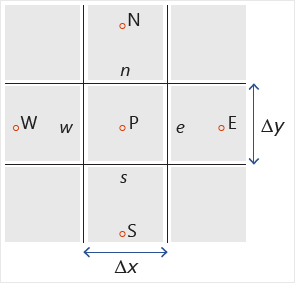
\includegraphics[scale=0.5]{2.png}
    \caption{有限體積的各個鄰計算點標號,以及各邊標號}
    \label{fig:1}
\end{figure}
\noindent figure1中,P點為當前計算點,亦為格點中心。P計算點,各有西東南北四個相鄰計算點分別為$(W\ E\ S\ N)$點,而有限體積相應於各個鄰計算點的邊分別為$(w\ e\ s\ n)$面,以此標號。\\
\newpage
\noindent 再利用$Gauss\ Divergence\ Theorem$,將式(15)轉為以下形式:\\
\begin{equation}
  \begin{split}
      \oint_{\partial \Omega(t)} \vec{da} \cdot T \vec{v} &=  \oint_{\partial \Omega(t)} \vec{da} \cdot  \alpha \vec{\nabla} T\\
  \end{split}
\end{equation}
\noindent 因此,對於$\Omega(t)$為二維平面矩形空間有:
\begin{equation}
  \begin{split}
      &\int_{\mbox{right}} dy \cdot T v_x(\vec{r} = right) - \int_{\mbox{left}} dy \cdot T v_x(\vec{r} = left) \\
      &+ \int_{\mbox{top}} dx \cdot T v_y(\vec{r} = top) - \int_{\mbox{bottom}} dx \cdot T v_y(\vec{r} = bottom) \\
      &=  \int_{\mbox{right}} dy  \cdot  \alpha \frac{\partial }{\partial x }  T(\vec{r} = right) - \int_{\mbox{left}} dy  \cdot  \alpha \frac{\partial }{\partial x }  T(\vec{r} = left) \\
      &+ \int_{\mbox{top}} dx  \cdot  \alpha \frac{\partial }{\partial y }  T(\vec{r} = top) - \int_{\mbox{bottom}} dx  \cdot  \alpha \frac{\partial }{\partial y }  T(\vec{r} = bottom) \\
  \end{split}
\end{equation}
\newpage
\noindent 三、空間二階精度中心離散格式\\

\noindent (一)、區域內點的一般離散格式\\

引入上式在有限體積之差分形式。進行四項近似,分別為:\\
\noindent 令p點$(i,j)$為有限體積之中心點,有限體積在西、東、南、北方之相鄰計算點分別為$(W\ ,E\ ,S\ ,N)$點,座標分別為$((i-1,j)\ ,(i+1,j)\ ,(i,j-1)\ ,(i,j+1))$,有限體積在西、東、南、北方之邊界上的中心點以$(w\ ,e\ ,s\ ,n)$表示,座標分別為$((i-\frac{1}{2},j)\ ,(i+\frac{1}{2},j)\ ,(i,j-\frac{1}{2})\ ,(i,j+\frac{1}{2}))$。\\
(1)各邊面積分化為中心點取值*積分範圍的大小\\
\noindent convection term:
\begin{equation}
\begin{split}
  \int_{\mbox{right}} dy \cdot T v_x(\vec{r} = right) = A_{e} \cdot T_{i+\frac{1}{2},j}v_{x\ i+\frac{1}{2},j}
\end{split}
\end{equation}
\noindent diffusion term:
\begin{equation}
\begin{split}
\int_{\mbox{right}} dy  \cdot  \alpha \vec{\nabla} T(\vec{r} = right) = A_{e} \cdot \alpha_{i+\frac{1}{2},j} (\frac{\partial}{\partial x} T)_{i+\frac{1}{2},j}
\end{split}
\end{equation}
\noindent 其中,$(A_{e},A_{w})$為有限體積在東、西方的邊界的大小,$(A_{s},A_{n})$為有限體積在南、北方的邊界的長度$(A_{s},A_{n})$。\\
\begin{minipage}[t]{0.45\textwidth}
  \raggedright
  (2)各個邊界上中心點的熱擴散係數為相鄰計算點(格點中心)之平均:
\begin{equation}
  \begin{split}
    \alpha_{i-\frac{1}{2},j} = \frac{\alpha_{i-1,j} + \alpha_{i,j}}{2}\\
    \alpha_{i+\frac{1}{2},j} = \frac{\alpha_{i,j} + \alpha_{i+1,j}}{2} \\
    \alpha_{i,j-\frac{1}{2}} = \frac{\alpha_{i,j-1} + \alpha_{i,j}}{2}\\
    \alpha_{i,j+\frac{1}{2}} = \frac{\alpha_{i,j} + \alpha_{i,j+1}}{2}\\
  \end{split}
\end{equation}
\end{minipage}
\hfill
\begin{minipage}[t]{0.45\textwidth}
  \raggedleft
  (3)各個邊界上中心點的溫度為相鄰計算點(格點中心)的溫度之平均:
  \begin{equation}
    \begin{split}
    T_{i-\frac{1}{2},j} = \frac{T_{i-1,j} + T_{i,j}}{2}\\
    T_{i+\frac{1}{2},j} = \frac{T_{i,j} + T_{i+1,j}}{2} \\
    T_{i,j-\frac{1}{2}} = \frac{T_{i,j-1} + T_{i,j}}{2}\\
    T_{i,j+\frac{1}{2}} = \frac{T_{i,j} + T_{i,j+1}}{2}\\
    \end{split}
  \end{equation}
\end{minipage}
\vspace{0.6em}

\noindent (4)個別邊界上中心點的溫度梯度沿外法線方向的分量取二階精度心插分:\\
\noindent ($A$($P$($E$($T$溫度)的(梯度))的(外法線分量))的(二階精度中心差分)):
\begin{equation}
  \begin{split}
    \mbox{西邊界中心點的中心差分:}\\
    (\frac{\partial}{\partial x} T)_{i-\frac{1}{2},j} = \frac{T_{i,j}-T_{i-1,j}}{\Delta x_{pW}} \\
    \mbox{東邊界中心點的中心差分:}\\
    (\frac{\partial}{\partial x} T)_{i+\frac{1}{2},j} = \frac{T_{i+1,j}-T_{i,j}}{\Delta x_{Ep}} \\
    \mbox{南邊界中心點的中心差分:}\\
    (\frac{\partial}{\partial y} T)_{i,j-\frac{1}{2}} = \frac{T_{i,j}-T_{i,j-1}}{\Delta y_{pS}} \\
    \mbox{北邊界中心點的中心差分:}\\
    (\frac{\partial}{\partial y} T)_{i,j+\frac{1}{2}} = \frac{T_{i,j+1}-T_{i,j}}{\Delta y_{Np}} \\
  \end{split}
\end{equation}
\noindent 其中,$\Delta x_{pW}$、$\Delta x_{Ep}$、$\Delta y_{pS}$、$\Delta y_{Np}$分別為中心點$p(i,j)$與$W(i-1,j)$、$E(i+1,j)$、$S(i,j-1)$、$N(i,j+1)$之相鄰格點中心點的距離。\\
\noindent 因此有:
\begin{equation}
\begin{split}
  &A_{e} \cdot \frac{T_{i,j} + T_{i+1,j}}{2} v_{x\ i+\frac{1}{2},j} - A_{w} \cdot \frac{T_{i-1,j} + T_{i,j}}{2} v_{x\ i-\frac{1}{2},j} \\
  &+ A_{n} \cdot \frac{T_{i,j} + T_{i,j+1}}{2} v_{y\ i,j+\frac{1}{2}} - A_{s} \cdot \frac{T_{i,j-1} + T_{i,j}}{2} v_{y\ i,j-\frac{1}{2}}\\
  &= A_{e} \cdot \frac{\alpha_{i,j} + \alpha_{i+1,j}}{2}\frac{T_{i+1,j}-T_{i,j}}{\Delta x_{Ep}}- A_{w} \cdot \frac{\alpha_{i-1,j} + \alpha_{i,j}}{2}\frac{T_{i,j}-T_{i-1,j}}{\Delta x_{pW}} \\
  &+ A_{n} \cdot \frac{\alpha_{i,j} + \alpha_{i,j+1}}{2}\frac{T_{i,j+1}-T_{i,j}}{\Delta y_{Np}} - A_{s} \cdot \frac{\alpha_{i,j-1} + \alpha_{i,j}}{2}\frac{T_{i,j}-T_{i,j-1}}{\Delta y_{pS}} \\
\end{split}
\end{equation}
\\上式即為不可壓縮裡想氣體的二維穩態擴散對流方程的空間二階精度中心離散格式。\\
\noindent 因此有:
\begin{equation}
\begin{split}
  &\frac{F_{e}}{2}(T_{p} + T_{E})-\frac{F_{w}}{2}(T_{W} + T_{p})+\frac{F_{n}}{2}(T_{N} + T_{p})-\frac{F_{s}}{2}(T_{S} + T_{p})\\
  & = D_{e} (T_{E}-T_{p} )- D_{w} (T_{p}-T_{W}) + D_{n} (T_{N}-T_{p}) - D_{s} (T_{p}-T_{S})\\
\end{split}
\end{equation}
\begin{equation}
\begin{split}
  &T_{p}\left[(D_{w}-\frac{F_{w}}{2})+(D_{e}+\frac{F_{e}}{2})+(D_{s}-\frac{F_{s}}{2})+(D_{n}+\frac{F_{n}}{2})\right] \\
  &= (D_{w}+\frac{F_{w}}{2})T_{W}+(D_{e}-\frac{F_{e}}{2})T_{E}+(D_{s}+\frac{F_{s}}{2})T_{S}+(D_{n}-\frac{F_{n}}{2})T_{N}
\end{split}
\end{equation}
\noindent 空間二階精度中心差分一般表達式為: 
\begin{equation}
\begin{split}
  &T_{p}\left[(D_{w}+\frac{F_{w}}{2})+(D_{e}-\frac{F_{e}}{2})+(D_{s}+\frac{F_{s}}{2})+(D_{n}-\frac{F_{n}}{2}) - F_{w} + F_{e} - F_{s} + F_{n} \right] \\
  &= (D_{w}+\frac{F_{w}}{2})T_{W}+(D_{e}-\frac{F_{e}}{2})T_{E}+(D_{s}+\frac{F_{s}}{2})T_{S}+(D_{n}-\frac{F_{n}}{2})T_{N}
\end{split}
\end{equation}
\noindent 其中,
\begin{equation}
\begin{split}
  &T_{W} = T_{i-1,j}\\
  &T_{E} = T_{i+1,j}\\
  &T_{S} = T_{i,j-1}\\
  &T_{N} = T_{i,j+1}\\
  &T_{P} = T_{i,j}\\
  &F_{w} = A_{w} v_{x\ i-\frac{1}{2},j}\\
  &F_{e} = A_{e} v_{x\ i+\frac{1}{2},j}\\
  &F_{s} = A_{s} v_{y\ i,j-\frac{1}{2}}\\
  &F_{n} = A_{n} v_{y\ i,j+\frac{1}{2}}\\
  &D_{w} = A_{w} \cdot \frac{\alpha_{i-1,j} + \alpha_{i,j}}{2\Delta x_{pW}}\\
  &D_{e} = A_{e} \cdot \frac{\alpha_{i,j} + \alpha_{i+1,j}}{2\Delta x_{Ep}}\\
  &D_{s} = A_{s} \cdot \frac{\alpha_{i,j-1} + \alpha_{i,j}}{2\Delta y_{pS}}\\
  &D_{n} = A_{n} \cdot \frac{\alpha_{i,j} + \alpha_{i,j+1}}{2\Delta y_{Np}}\\
\end{split}
\end{equation}

\noindent (二)、邊界處理之算例:\\

\noindent (1)將非齊性邊界條件視為外源項,放入$S_{u}\ S_{p}$中。\\
若對於$p(i,j)$點,其西邊界重合於physical boundary ,則對於$p(i,j)$,不可壓縮裡想氣體的二維穩態擴散對流方程的空間二階精度中心離散格式為:\\
\noindent [通用式]: 
\begin{equation}
\begin{split}
  &A_{e} \cdot \frac{T_{i,j} + T_{i+1,j}}{2} v_{x\ i+\frac{1}{2},j} - 0 \\
  &+ A_{n} \cdot \frac{T_{i,j} + T_{i,j+1}}{2} v_{y\ i,j+\frac{1}{2}} - A_{s} \cdot \frac{T_{i,j-1} + T_{i,j}}{2} v_{y\ i,j-\frac{1}{2}}- A_{w} \cdot T_{i-\frac{1}{2},j}v_{x\ i-\frac{1}{2},j} \\
  &= A_{e} \cdot \frac{\alpha_{i,j} + \alpha_{i+1,j}}{2}\frac{T_{i+1,j}-T_{i,j}}{\Delta x_{Ep}}- 0 \\
  &+ A_{n} \cdot \frac{\alpha_{i,j} + \alpha_{i,j+1}}{2}\frac{T_{i,j+1}-T_{i,j}}{\Delta y_{Np}} - A_{s} \cdot \frac{\alpha_{i,j-1} + \alpha_{i,j}}{2}\frac{T_{i,j}-T_{i,j-1}}{\Delta y_{pS}} - A_{w} \cdot \alpha_{i-\frac{1}{2},j} \frac{T_{i,j}-T_{i-\frac{1}{2},j}}{\Delta x_{pW}}\\
\end{split}
\end{equation}
\noindent 也可以寫成: 
\begin{equation}
\begin{split}
  &\frac{F_{e}}{2}(T_{p} + T_{E})- 0 +\frac{F_{n}}{2}(T_{N} + T_{p})-\frac{F_{s}}{2}(T_{S} + T_{p}) - A_{w} \cdot T_{i-\frac{1}{2},j}v_{x\ i-\frac{1}{2},j} \\
  & = D_{e} (T_{E}-T_{p} ) - 0 + D_{n} (T_{N}-T_{p}) - D_{s} (T_{p}-T_{S}) - A_{w} \cdot \alpha_{i-\frac{1}{2},j} \frac{T_{i,j}-T_{i-\frac{1}{2},j}}{\Delta x_{pW}}
\end{split}
\end{equation}
\noindent p點為整個定義域的左邊界計算點。
\noindent [通用公式]:
\begin{equation}
\begin{split}
  &T_{p}\left[(D_{w}+\frac{F_{w}}{2})+(D_{e}-\frac{F_{e}}{2})+(D_{s}+\frac{F_{s}}{2})+(D_{n}-\frac{F_{n}}{2}) - F_{w} + F_{e} - F_{s} + F_{n}  - S_{p}\right] \\
  &= (D_{w}+\frac{F_{w}}{2})T_{W}+(D_{e}-\frac{F_{e}}{2})T_{E}+(D_{s}+\frac{F_{s}}{2})T_{S}+(D_{n}-\frac{F_{n}}{2})T_{N} + S_{u}
\end{split}
\end{equation}
\vspace{-0.7em}
\noindent 其中,
\begin{equation}
  \begin{split}
    &T_{p} = T_{i,j}\\
    &T_{W} = 0.0 ;\\
    &T_{E} = T_{i+1,j} \\
    &T_{S} = T_{i,j-1} \\
    &T_{N} = T_{i,j+1}\\
    &F_{w} = 0 \\
    &F_{e} = A_{e}v_{i+\frac{1}{2},j}\\
    &F_{s} = A_{s}v_{i,j-\frac{1}{2}}\\
    &F_{n} = A_{n}v_{i,j+\frac{1}{2}}\\
    &D_{w} = 0\\
    &D_{e} = A_{e} \frac{\alpha_{i,j}+\alpha_{i+1,j}}{2\Delta x_{Ep}}\\
    &D_{s} = A_{s} \frac{\alpha_{i,j-1}+\alpha_{i,j}}{2\Delta y_{pS}}\\
    &D_{n} = A_{n} \frac{\alpha_{i,j}+\alpha_{i,j+1}}{2\Delta y_{Np}}\\
    &S_{p} = -\frac{A_{w}\alpha_{i-\frac{1}{2},j}}{\Delta x_{pw}}\\
    &S_{u} = (A_{w} v_{x\ i-\frac{1}{2},j} + \frac{A_{w}\alpha_{i-\frac{1}{2},j}}{\Delta x_{pw}})T_{i-\frac{1}{2},j}\\
  \end{split}
\end{equation}
\noindent 再次計算另外一個算例:\\
(2)若對於$p(i,j)$點,其北邊界重合於physical boundary ,則對於$p(i,j)$,不可壓縮裡想氣體的二維穩態擴散對流方程的空間二階精度中心離散格式為:\\
\noindent [通用式]: 
\begin{equation}
\begin{split}
  &A_{e} \cdot \frac{T_{i,j} + T_{i+1,j}}{2} v_{x\ i+\frac{1}{2},j} - A_{w} \cdot \frac{T_{i-1,j} + T_{i,j}}{2} v_{x\ i-\frac{1}{2},j} \\
  &+ 0 - A_{s} \cdot \frac{T_{i,j-1} + T_{i,j}}{2} v_{y\ i,j-\frac{1}{2}} + A_{n} \cdot T_{i,j+\frac{1}{2}}v_{x\ i,j+\frac{1}{2}} \\
  &= A_{e} \cdot \frac{\alpha_{i,j} + \alpha_{i+1,j}}{2}\frac{T_{i+1,j}-T_{i,j}}{\Delta x_{Ep}}- A_{w} \cdot \frac{\alpha_{i-1,j} + \alpha_{i,j}}{2}\frac{T_{i,j}-T_{i-1,j}}{\Delta x_{pW}} \\
  &+ 0 - A_{s} \cdot \frac{\alpha_{i,j-1} + \alpha_{i,j}}{2}\frac{T_{i,j}-T_{i,j-1}}{\Delta y_{pS}} + A_{n} \cdot \alpha_{i,j+\frac{1}{2}} \frac{T_{i,j+\frac{1}{2}}-T_{i,j}}{\Delta y_{ns}} \\
\end{split}
\end{equation}
\noindent 也可以寫成: 
\begin{equation}
\begin{split}
  &\frac{F_{e}}{2}(T_{p} + T_{E})- \frac{F_{w}}{2}(T_{p} + T_{W})+ 0 -\frac{F_{s}}{2}(T_{S} + T_{p}) + A_{n} \cdot T_{i,j+\frac{1}{2}}v_{x\ i,j+\frac{1}{2}} \\
  & = D_{e} (T_{E}-T_{p} ) - D_{w}(T_{p} - T_{W}) + 0  - D_{s} (T_{p}-T_{S}) + A_{n} \cdot \alpha_{i,j+\frac{1}{2}} \frac{T_{i,j+\frac{1}{2}}-T_{i,j}}{\Delta y_{ns}}
\end{split}
\end{equation}
\noindent 其中,p點為整個定義域的上邊界計算點。[通用公式]:
\begin{equation}
\begin{split}
  &T_{p}\left[(D_{w}+\frac{F_{w}}{2})+(D_{e}-\frac{F_{e}}{2})+(D_{s}+\frac{F_{s}}{2})+(D_{n}-\frac{F_{n}}{2}) - F_{w} + F_{e} - F_{s} + F_{n}  - S_{p}\right] \\
  &= (D_{w}+\frac{F_{w}}{2})T_{W}+(D_{e}-\frac{F_{e}}{2})T_{E}+(D_{s}+\frac{F_{s}}{2})T_{S}+(D_{n}-\frac{F_{n}}{2})T_{N} + S_{u}
\end{split}
\end{equation}
\noindent 其中,
\begin{equation}
  \begin{split}
    &T_{p} = T_{i,j}\\
    &T_{W} = T_{i-1,j} ;\\
    &T_{E} = T_{i+1,j} \\
    &T_{S} = 0 \\
    &T_{N} = T_{i,j+1}\\
    &F_{w} =  A_{w}v_{x\ i-\frac{1}{2},j}\\
    &F_{e} = A_{e}v_{i+\frac{1}{2},j}\\
    &F_{s} = A_{s}v_{i,j-\frac{1}{2}}\\
    &F_{n} = 0\\
    &D_{w} = A_{w}\frac{\alpha_{i-1,j} + \alpha_{i,j}}{2\Delta x_{pW}}\\
    &D_{e} = A_{e} \frac{\alpha_{i,j}+\alpha_{i+1,j}}{2\Delta x_{Ep} }\\
    &D_{s} = A_{s} \frac{\alpha_{i,j-1}+\alpha_{i,j}}{2\Delta y_{pS}}\\
    &D_{n} = 0\\
    &S_{p} = -\frac{A_{n}\alpha_{i,j+\frac{1}{2}}}{\Delta y_{np}}\\
    &S_{u} = (-A_{n} v_{x\ i,j+\frac{1}{2}} + \frac{A_{n}\alpha_{i,j+\frac{1}{2}}}{\Delta y_{np}})T_{i,j+\frac{1}{2}}\\
  \end{split}
\end{equation}
\noindent (三)、assignment 2之條件下的邊界計算點所滿足的方程式:\\

\noindent (三-1)左邊界:\\

(1)範圍:$(i = 0 ; j = 1 : Ny - 2)$,(2)溫度邊界條件$T_{-\frac{1}{2},j} = 1.0$,(3)速度條件:$(u = 1.0 ; v = 1.0)$ for every node

\begin{equation}
  \begin{split}
    &\frac{dy}{2}(T_{0,j}+T_{1,j}) - 0 + \frac{dx}{2}(T_{0,j}+T_{0,j+1}) - \frac{dx}{2}(T_{0,j}+T_{0,j-1}) \\ -&  dyT_{-\frac{1}{2},j} \\
    = &\alpha \cdot (T_{1,j} - T_{0,j}) - 0 + \alpha \cdot (T_{0,j+1} - T_{0,j}) -\alpha \cdot (T_{0,j} - T_{0,j-1}) \\-& 2 \alpha (T_{0,j} - T_{-\frac{1}{2} , j}) \\
  \end{split}
\end{equation}
\noindent 進一步可以寫成:

\begin{equation}
  \begin{split}
    &T_{0,j}(\frac{dy}{2}+5\alpha )\\
    =& 0 + T_{1,j}(-\frac{dy}{2}+\alpha)+ T_{0,j-1}(\frac{dx}{2}+\alpha)+T_{0,j+1}(-\frac{dx}{2}+\alpha)\\+&T_{-\frac{1}{2},j}(dy+2\alpha) \\
  \end{split}
\end{equation}

\noindent (三-2)右邊界:\\

(1)範圍:$(i = Nx-1 ; j = 1 : Ny - 2)$,(2)溫度邊界條件$T_{Nx-\frac{1}{2},j} = 0.0$,(3)速度條件:$(u = 1.0 ; v = 1.0)$ for every node\\
\begin{equation}
  \begin{split}
    &0-\frac{dy}{2}(T_{Nx-1,j}+T_{Nx-2,j}) + \frac{dx}{2}(T_{Nx-1,j+1}+T_{Nx-1,j}) - \frac{dx}{2}(T_{Nx-1,j}+T_{Nx-1,j-1}) \\+&  dyT_{Nx-\frac{1}{2},j} \\
    = &0-\alpha \cdot (T_{Nx-1,j}-T_{Nx-2,j}) + \alpha \cdot (T_{Nx-1,j+1} - T_{Nx-1,j}) -\alpha \cdot (T_{Nx-1,j} - T_{Nx-1,j-1}) \\ 
    + &2 \alpha (T_{Nx-\frac{1}{2} , j}-T_{Nx-1,j}) \\
  \end{split}
\end{equation}
\noindent 進一步可以寫成:\\
\begin{equation}
  \begin{split}
    &T_{Nx-1,j}(-\frac{dy}{2}+5\alpha )\\
    =&T_{Nx-2,j}(\frac{dy}{2}+\alpha) + 0 +T_{Nx-1,j-1}(\frac{dx}{2}+\alpha)+T_{Nx-1,j+1}(-\frac{dx}{2}+\alpha)\\
    +&T_{Nx-\frac{1}{2},j}(-dy+2\alpha) \\
  \end{split}
\end{equation}

\noindent (三-3)下邊界:\\

(1)範圍:$(i = 1 : Nx-1 ; j = 0)$,(2)溫度邊界條件$T_{i,-\frac{1}{2}} = 0.0$,(3)速度條件:$(u = 1.0 ; v = 1.0)$ for every node\\
\begin{equation}
  \begin{split}
    &\frac{dy}{2}(T_{i+1,0,}+T_{i,0})-\frac{dy}{2}(T_{i-1,0}+T_{i,0}) + \frac{dx}{2}(T_{i,1}+T_{i,0}) - 0 \\-& dx T_{i,-\frac{1}{2}} \\
    = &\alpha \cdot (T_{i+1,0}-T_{i,0})-\alpha \cdot (T_{i,0}-T_{i-1,0}) + \alpha \cdot (T_{i,1} - T_{i,0}) -0 \\-& 2\alpha(T_{i,0}-T_{i,-\frac{1}{2}}) \\ 
  \end{split}
\end{equation}
\noindent 進一步可以寫成:\\
\begin{equation}
  \begin{split}
    &T_{i,0}(\frac{dx}{2}+5\alpha )\\
    =&T_{i-1,0}(\frac{dy}{2}+\alpha) +T_{i+1,0}(-\frac{dy}{2}+\alpha) +0 +T_{i,1}(-\frac{dx}{2}+\alpha)\\
    +&T_{i,-\frac{1}{2}}(dx+2\alpha) \\
  \end{split}
\end{equation}

\noindent (三-4)上邊界:\\

(1)範圍:$(i = 1 : Nx-1 ; j = Ny-1)$,(2)溫度邊界條件$T_{i,Ny-\frac{1}{2}} = 1.0$,(3)速度條件:$(u = 1.0 ; v = 1.0)$ for every node\\
\begin{equation}
  \begin{split}
    &\frac{dy}{2}(T_{i+1,Ny-1}+T_{i,Ny-1})-\frac{dy}{2}(T_{i-1,Ny-1}+T_{i,Ny-1}) + 0 - \frac{dx}{2}(T_{i,Ny-1} + T_{i,Ny-2}) \\+& dx T_{i,Ny-\frac{1}{2}} \\
    = &\alpha \cdot (T_{i+1,Ny-1}-T_{i,Ny-1})-\alpha \cdot (T_{i,Ny-1}-T_{i-1,Ny-1})+ 0 - \alpha (T_{i,Ny-1}-T_{i,Ny-2}) \\+& 2\alpha(T_{i,Ny-\frac{1}{2}} - T_{i,Ny-1}) \\ 
  \end{split}
\end{equation}
\noindent 進一步可以寫成:\\
\begin{equation}
  \begin{split}
    &T_{i,Ny-1}(-\frac{dx}{2}+5\alpha )\\
    =&T_{i-1,Ny-1}(\frac{dy}{2}+\alpha) +T_{i+1,Ny-1}(-\frac{dy}{2}+\alpha) + T_{i,Ny-2}(\frac{dx}{2}+\alpha) + 0 \\
    +&T_{i,Ny-\frac{1}{2}}(-dx+2\alpha) \\
  \end{split}
\end{equation}
\vspace{0.6em}

以上即為"不可壓縮流理想氣體的二維穩態擴散對流方程的空間二階精度中心差分離散格式“。\\
\newpage
\noindent 四、空間三階精度迎風型QUICK離散格式\\

在不可壓縮流理想氣體的二維穩態擴散對流方程的空間二階精度中心差分離散格式的基礎上,進行空間三階精度迎風型QUICK離散格式的推導。
\noindent QUICK離散格式為處理有限體積法中,對流項中的溫度場在邊界中心點的取值近似問題。\\

\noindent QUICK離散格式有兩大重點:\\
\noindent  (1) ($Q$($W$($E$($I$有限體積)的(邊界))的(中心點))的(溫度))的近似\\
\noindent  (2) ($U$($W$($E$($I$有限體積)的(邊界))的(中心點))的(溫度梯度))的近似,在邊界計算點特殊近似。\\
\begin{figure}[H]
  \centering
  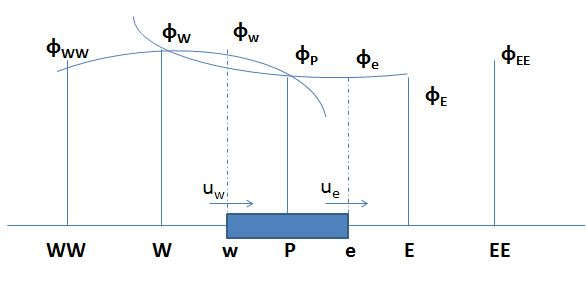
\includegraphics[scale = 0.5]{3.jpg}
  \caption{QUICK scheme}
  \label{fig:QUICK}
\end{figure}
\begin{figure}[H]
    \centering
    \begin{minipage}{0.45\textwidth}
        \centering
        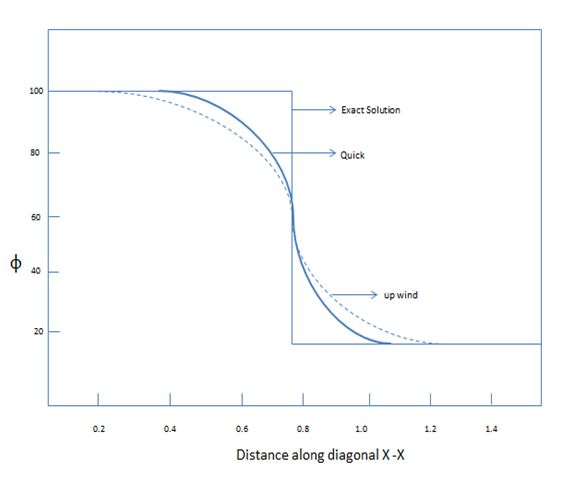
\includegraphics[width=\textwidth, height=6cm]{8.jpg}
        \caption{compare QUICK scheme 以及 upwind scheme}
        \label{fig:quick1}
    \end{minipage}
    \hfill
    \begin{minipage}{0.45\textwidth}
        \centering
        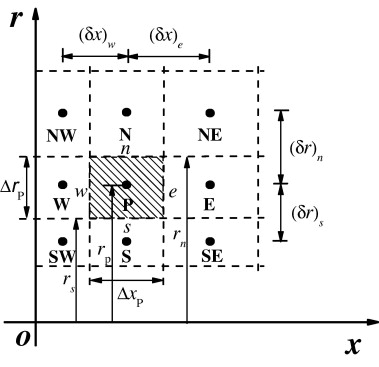
\includegraphics[width=\textwidth, height=6cm]{4.jpg}
        \caption{finit volume method}
        \label{fig:quick2}
    \end{minipage}
\end{figure}
\noindent (一)、內格子點在各邊界中心點的溫度取值\\

現在給出QUICK離散格式在有限體積(令此有限體積的中心點$p(i,j)$)在各個邊界的溫度取值,以及在各個不同條件下的形式。\\
\noindent 溫度場$T$在以$p$點為中心點的格點的西邊界中心點的取值\\
\begin{equation}
\begin{split}
  T_{i-\frac{1}{2},j} = B_{w}(\frac{6}{8}T_{i-1,j}+\frac{3}{8}T_{i,j}-\frac{1}{8}T_{i-2,j})+C_{w}(\frac{6}{8}T_{i,j}+\frac{3}{8}T_{i-1,j}-\frac{1}{8}T_{i+1,j})\\
\end{split}
\end{equation}
\begin{equation}
\begin{split}
  T_{i-\frac{1}{2},j} = \frac{1}{8}\left((6B_{w}+3C_{w})T_{i-1,j}+(3B_{w}+6C_{w})T_{i,j}+(-B_{w})T_{i-2,j}+(-C_{w})T_{i+1,j}\right)\\
\end{split}
\end{equation}
\noindent 其中,當$F_{w} = A_{w}u_{i-\frac{1}{2},j}>0$時,$B_{w} = 1.0$且$C_{w} = 0.0$;當$F_{w} = A_{w}u_{i-\frac{1}{2},j}<0$時,$B_{w} = 0.0$且$C_{w} = 1.0$。\\
\noindent 溫度場$T$在以$p$點為中心點的格子的東邊界中心點的取值\\
\begin{equation}
\begin{split}
  T_{i+\frac{1}{2},j} = B_{e}(\frac{6}{8}T_{i,j}+\frac{3}{8}T_{i+1,j}-\frac{1}{8}T_{i-1,j})+C_{e}(\frac{6}{8}T_{i+1,j}+\frac{3}{8}T_{i,j}-\frac{1}{8}T_{i+2,j})\\
\end{split}
\end{equation}
\begin{equation}
\begin{split}
    T_{i+\frac{1}{2},j} = \frac{1}{8}\left((6B_{e}+3C_{e})T_{i,j}+(3B_{e}+6C_{e})T_{i+1,j}+(-B_{w})T_{i-1,j}+(-C_{w})T_{i+2,j}\right)\\
\end{split}
\end{equation}
\noindent 其中,當$F_{e} = A_{e}u_{i+\frac{1}{2},j}>0$時,$B_{e} = 1.0$且$C_{e} = 0.0$;當$F_{e} = A_{e}u_{i+\frac{1}{2},J}<0$時,$B_{e} = 0.0$且$C_{e} = 1.0$。\\
\noindent 溫度場$T$在以$p$點為中心點的格子的南邊界中心點的取值\\
\begin{equation}
\begin{split}
  T_{i,j-\frac{1}{2}} = B_{s}(\frac{6}{8}T_{i,j-1}+\frac{3}{8}T_{i,j}-\frac{1}{8}T_{i,j-2})+C_{s}(\frac{6}{8}T_{i,j}+\frac{3}{8}T_{i,j-1}-\frac{1}{8}T_{i,j+1})
\end{split}
\end{equation}
\begin{equation}
\begin{split}
  T_{i,j-\frac{1}{2}} = \frac{1}{8}\left((6B_{s}+3C_{s})T_{i,j-1}+(3B_{s}+6C_{s})T_{i,j}+(-B_{s})T_{i,j-2}+(-C_{s})T_{i,j+1}\right)\\
\end{split}
\end{equation}
\noindent 其中,當$F_{s} = A_{s}u_{i,j-\frac{1}{2}}>0$時,$B_{s} = 1.0$且$C_{s} = 0.0$;當$F_{s} = A_{s}u_{i,j-\frac{1}{2}}<0$時,$B_{s} = 0.0$且$C_{s} = 1.0$。\\
\noindent 溫度$T$在以$p$的點為中心點的格子的北邊界中心點的取值:
\begin{equation}
\begin{split}
  T_{i,j+\frac{1}{2}} = B_{n}(\frac{6}{8}T_{i,j}+\frac{3}{8}T_{i,j+1}-\frac{1}{8}T_{i,j-1})+C_{n}(\frac{6}{8}T_{i,j+1}+\frac{3}{8}T_{i,j}-\frac{1}{8}T_{i,j+2})
\end{split}
\end{equation}
\begin{equation}
\begin{split}
  T_{i,j+\frac{1}{2}} = \frac{1}{8}\left((6B_{n}+3C_{n})T_{i,j}+(3B_{n}+6C_{n})T_{i,j+1}+(-B_{n})T_{i,j-1}+(-C_{n})T_{i,j+2}\right)\\
\end{split}
\end{equation}
\noindent 其中,當$F_{n} = A_{n}u_{i,j+\frac{1}{2}}>0$時,$B_{n} = 1.0$且$C_{n} = 0.0$;當$F_{n} = A_{n}u_{i,j+\frac{1}{2}}<0$時,$B_{n} = 0.0$且$C_{n} = 1.0$。\\

若將$(36)(38)(40)(42)$取代式$(22)$,且將其他近似項$(19)(20)(21)(23)$保留,則不可壓縮理想氣體的二維穩態擴散對流方程的積分形式的空間三階精度迎風型QUICK離散格式為:
\begin{equation}
\begin{split}
  &A_{e} \cdot \frac{1}{8}\left((6B_{e}+3C_{e})T_{i,j}+(3B_{e}+6C_{e})T_{i+1,j}+(-B_{w})T_{i-1,j}+(-C_{w})T_{i+2,j}\right) v_{x\ i+\frac{1}{2},j} \\
  - &A_{w} \cdot \frac{1}{8}\left((6B_{w}+3C_{w})T_{i-1,j}+(3B_{w}+6C_{w})T_{i,j}+(-B_{w})T_{i-2,j}+(-C_{w})T_{i+1,j}\right) v_{x\ i-\frac{1}{2},j} \\
  + &A_{n} \cdot \frac{1}{8}\left((6B_{n}+3C_{n})T_{i,j}+(3B_{n}+6C_{n})T_{i,j+1}+(-B_{n})T_{i,j-1}+(-C_{n})T_{i,j+2}\right) v_{y\ i,j+\frac{1}{2}} \\
  - &A_{s} \cdot \frac{1}{8}\left((6B_{s}+3C_{s})T_{i,j-1}+(3B_{s}+6C_{s})T_{i,j}+(-B_{s})T_{i,j-2}+(-C_{s})T_{i,j+1}\right) v_{y\ i,j-\frac{1}{2}}\\
  = &A_{e} \cdot \frac{\alpha_{i,j} + \alpha_{i+1,j}}{2}\frac{T_{i+1,j}-T_{i,j}}{\Delta x_{Ep}}- A_{w} \cdot \frac{\alpha_{i-1,j} + \alpha_{i,j}}{2}\frac{T_{i,j}-T_{i-1,j}}{\Delta x_{pW}} \\
  + &A_{n} \cdot \frac{\alpha_{i,j} + \alpha_{i,j+1}}{2}\frac{T_{i,j+1}-T_{i,j}}{\Delta y_{Np}} - A_{s} \cdot \frac{\alpha_{i,j-1} + \alpha_{i,j}}{2}\frac{T_{i,j}-T_{i,j-1}}{\Delta y_{pS}} \\
\end{split}
\end{equation}
\noindent 上式即為內計算點所應該滿足的空間三階精度QUICK離散格式。\\

由assignment2給定的條件可知,$(B_{w},B_{e},B_{s},B_{n}) = (1,1,1,1)$且$(C_{w},C_{e},C_{s},C_{n}) = (0,0,0,0 )$,也就是說每一個網格階做一樣的事情,以及每一格網格的邊界中心點的速度都$>0$,且此題假設均勻正方形網格,因此定義域中每個網格邊長$A_{w} = A_{e} = A_{s} = A_{n} = \Delta x = \Delta y$,且熱擴散係數$\alpha$為全場均勻,且非時變,因此可以簡化如下:\\
\noindent 內點:
\begin{equation}
\begin{split}
     &T_{i,j}(4\alpha+\Delta y \frac{3}{8}+\Delta x \frac{3}{8})\\
   = &T_{i-1,j}(\alpha+\Delta y \frac{7}{8})+T_{i+1,j}(\alpha-\Delta y \frac{3}{8})+T_{i,j-1}(\alpha + \Delta x \frac{7}{8} )+T_{i,j+1}(\alpha - \Delta x \frac{3}{8})\\
   + &T_{i-2,j}(-\Delta y \frac{1}{8})+T_{i,j-2}(-\Delta x \frac{1}{8})
\end{split}
\end{equation}
\noindent 通用表示式:不可壓縮理想氣體的二維穩態擴散對流方程的積分形式的空間三階精度QUICK離散格式:在速度條件為$u = 1.0\ v = 1.0$的條件下亦有如下形式:\\
\begin{equation}
  \begin{split}
    a_{p}T_{p} = a_{W}T_{W}+a_{E}T_{E}+a_{WW}T_{WW}+a_{S}T_{S}+a_{N}T_{N}+a_{SS}T_{SS}
  \end{split}
\end{equation}
\begin{table}[H]
    \centering
    \begin{tabular}{|c|c|c|c|}
        \hline
        通用係數&$a_{W}$ & $a_{E}$ & $a_{WW}$ \\
        \hline
        表達式&$D_{w}+\frac{6}{8}F_{w}+\frac{1}{8}F_{e}$ & $D_{e}-\frac{3}{8}F_{e}$ & $-\frac{1}{8}F_{w}$\\
        \hline
         通用係數&$a_{S}$ & $a_{N}$ & $a_{SS}$ \\
        \hline
        表達式&$D_{s}+\frac{6}{8}F_{s}+\frac{1}{8}F_{n}$ & $D_{n}-\frac{3}{8}F_{n}$ & $-\frac{1}{8}F_{s}$\\
        \hline
         通用係數&$a_{p}$ &  &  \\
        \hline
        表達式&$\left[a_{W}+a_{E}+a_{WW}+F_{e}-F_{w}\right]+\left[a_{S}+a_{N}+a_{SS}+F_{n}-F_{s}\right]$ & &\\
        \hline
    \end{tabular}
    \caption{QUICK coefficients}
    \label{tab:general_QUICK_coefficients}
\end{table}
\begin{table}[H]
    \centering
    \begin{tabular}{|c|c|c|c|c|c|c|c|}
        \hline
        溫度簡寫&$T_{p}$&$T_{W}$& $T_{E}$ & $T_{WW}$&$T_{S}$&$T_{N}$& $T_{SS}$ \\
        \hline
        離散座標溫度&$T_{i,j}$&$T_{i-1,j}$& $T_{i+1,j}$ & $T_{i-2,j}$&$T_{i,j-1}$&$T_{i,j+1}$& $T_{i,j-2}$ \\
        \hline
    \end{tabular}
    \caption{discreted temperature}
    \label{tab:general_discreted_temperature}
\end{table}
\begin{table}[H]
    \centering
    \begin{tabular}{|c|c|c|c|}
        \hline
        內係數簡寫&$F_{w}$&$D_{w}$& $\alpha_{i-\frac{1}{2},j}$ \\ 
        \hline
        表達式&$A_{w}u_{i-\frac{1}{2},j}$&$A_{w}\frac{\alpha_{i-\frac{1}{2},j}}{\Delta x_{pW}}$& $\frac{\alpha_{i-1,j}+\alpha_{i,j}}{2}$ \\
        \hline
    \end{tabular}
    \caption{$D_{w},F_{w},\alpha_{i-\frac{1}{2},j}$表達式,其他有限體積值之邊界亦然}
    \label{tab:1D_e_F_e_alpha}
\end{table}
\begin{table}[H]
    \centering
    \begin{tabular}{|c|c|c|c|}
        \hline
        內係數簡寫&$F_{e}$&$D_{e}$& $\alpha_{i+\frac{1}{2},j}$ \\ 
        \hline
        表達式&$A_{e}u_{i+\frac{1}{2},j}$&$A_{e}\frac{\alpha_{i+\frac{1}{2},j}}{\Delta x_{Ep}}$& $\frac{\alpha_{i+1,j}+\alpha_{i,j}}{2}$ \\
        \hline
    \end{tabular}
    \caption{$D_{e},F_{e},\alpha_{i+\frac{1}{2},j}$表達式,其他有限體積值之邊界亦然}
    \label{tab:2D_e_F_e_alpha}
\end{table}
\begin{table}[H]
    \centering
    \begin{tabular}{|c|c|c|c|}
        \hline
        內係數簡寫&$F_{s}$&$D_{s}$& $\alpha_{i,j-\frac{1}{2}}$ \\ 
        \hline
        表達式&$A_{s}u_{i,j-\frac{1}{2}}$&$A_{s}\frac{\alpha_{i,j-\frac{1}{2}}}{\Delta y_{pS}}$& $\frac{\alpha_{i,j-1}+\alpha_{i,j}}{2}$ \\
        \hline
    \end{tabular}
    \caption{$D_{s},F_{s},\alpha_{i,j-\frac{1}{2}}$表達式,其他有限體積值之邊界亦然}
    \label{tab:D_e_F_e_alpha}
\end{table}
\begin{table}[H]
    \centering
    \begin{tabular}{|c|c|c|c|}
        \hline
        內係數簡寫&$F_{n}$&$D_{n}$& $\alpha_{i,j+\frac{1}{2}}$ \\ 
        \hline
        表達式&$A_{n}u_{i,j+\frac{1}{2}}$&$A_{n}\frac{\alpha_{i,j+\frac{1}{2}}}{\Delta y_{Np}}$& $\frac{\alpha_{i,j+1}+\alpha_{i,j}}{2}$ \\
        \hline
    \end{tabular}
    \caption{$D_{n},F_{n},\alpha_{i,j+\frac{1}{2}}$表達式,其他有限體積值之邊界亦然}
    \label{tab:3D_e_F_e_alpha}
\end{table}
\newpage
\noindent (二)、邊界處理之算例:\\
\noindent 針對對流項中,邊界中心點的溫度處理:此題邊界條件採用Dirichelet Boundary Condition。\\
\noindent 將非齊性邊界條件之影響放入外源項中,通用格式有:
\begin{equation}
  \begin{split}
    a_{p}T_{p} = a_{W}T_{W}+a_{E}T_{E}+a_{WW}T_{WW}+a_{S}T_{S}+a_{N}T_{N}+a_{SS}T_{SS} + S_{u}\\
  \end{split}
\end{equation}
\noindent 其中,$$a_{p} = a_{W}+a_{E}+a_{WW}-F_{w}+F_{e}+a_{S}+a_{N}+a_{SS}-F_{s}+F_{n}-S_{p}$$\\
\noindent 通用格式亦可以寫成如下:
\begin{equation}
  \begin{split}
    &((D_{w}+\frac{6}{8}F_{w}+\frac{1}{8}F_{e})+(D_{e}-\frac{3}{8}F_{e})+(\frac{1}{8}F_{e})-F_{w}+F_{e}\\
    &+(D_{s}+\frac{6}{8}F_{s}+\frac{1}{8}F_{n})+(D_{n}-\frac{3}{8}F_{n})+(\frac{1}{8}F_{n})-F_{s}+F_{n}-S_{p})T_{p}\\
    =&(D_{w}+\frac{6}{8}F_{w}+\frac{1}{8}F_{e})T_{W}+(D_{e}-\frac{3}{8}F_{e})T_{E}+(\frac{1}{8}F_{e})T_{WW}\\
    &+(D_{s}+\frac{6}{8}F_{s}+\frac{1}{8}F_{n})T_{S}+(D_{n}-\frac{3}{8}F_{n})T_{N}+(\frac{1}{8}F_{n})T_{SS} \\
    &+S_{u}
  \end{split}
\end{equation}
\noindent 可配合邊界條件更改外源項$S_{p}$、$S_{u}$。\\
在空間三階精度QUICK離散格式中,邊界處理的節點有,整個平面區域之上下左右第一排邊界計算點以及根據速度場$u = 1.0 \  v = 1.0$,之方向,下、左第二排邊界計算點需要做邊界處理。
其中,(1)對於左邊界第一排計算點的西側邊界、右邊界第一排計算點的東側邊界、下邊界第一排計算點的南側邊界、上邊界第一排計算點的北側邊界,其中心點的溫度場由邊界條件直接賦值。
(2)對於左邊界第一排計算點的東側邊界、右邊界第一排計算點的西側邊界、下邊界第一排計算點的北側邊界、上邊界第一排計算點的南側邊界、左邊界第二排計算點的西側邊界、下邊界第二排計算點的南側邊界,其中心點的溫度場由線性差值賦值。\\
\noindent 由Leonard(1979)提供的建議,對於用到邊界後面不存在的節點(格點)溫度場,採用線性外插的方式:
\begin{figure}[H]
  \centering
  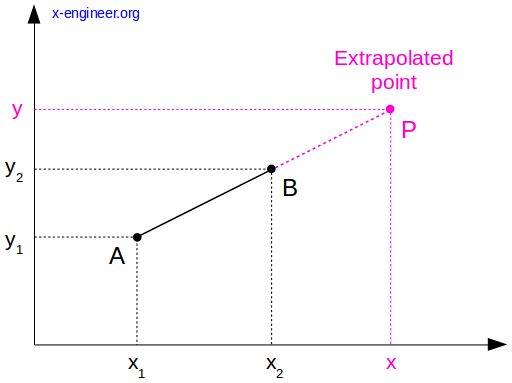
\includegraphics[scale = 0.5]{5.png}
  \caption{Leonard提議採用 Linear extrapolation處理邊界外計算點的溫度場}
  \label{fig:Linear_extrapolation}
\end{figure}
\noindent 外插計算的溫度場$T_{P}$滿足如下形式:
$$
  T_{P} = 2T_{B} - T_{A} = 2T_{physical\ boundary} - T_{computational\ boundary}
$$
\noindent (二-1)各邊界計算點的外邊界:由邊界條件直接給定:\\

\noindent (二-1.1)左邊界第一排計算點的西側邊界:$$T_{-\frac{1}{2},j} = 1.0$$\\
\noindent (二-1.2)右邊界第一排計算點的東側邊界:$$T_{Nx-\frac{1}{2},j} = 0.0$$\\
\noindent (二-1.3)下邊界第一排計算點的南側邊界:$$T_{i,-\frac{1}{2}} = 0.0$$\\
\noindent (二-1.4)上邊界第一排計算點的北側邊界:$$T_{i,Ny-0\frac{1}{2}} = 1.0$$\\
\noindent (二-2)配合迎風條件,有限體積邊界中心點的對流項溫度的線性外插:(由給定之速度場$u = 1.0 , v = 1.0$,對於每一個格點):\\

\noindent (二-2.1)左邊界第一排計算點的東側邊界:$$T_{\frac{1}{2},j} = \frac{6}{8}T_{0,j}+\frac{3}{8}T_{1,j}-\frac{1}{8}T_{-1,j}^{*} =\frac{7}{8}T_{0,j}+\frac{3}{8}T_{1,j}-\frac{2}{8}T_{-\frac{1}{2},j}  $$\\
\noindent (二-2.2)下邊界第一排計算點的北側邊界:$$T_{i,\frac{1}{2}} = \frac{6}{8}T_{i,0}+\frac{3}{8}T_{i,1}-\frac{1}{8}T_{i,-1}^{*} = \frac{7}{8}T_{i,0}+\frac{3}{8}T_{i,1}-\frac{2}{8}T_{i,-\frac{1}{2}}$$\\
\noindent (二-2.3)左邊界第二排計算點的西側邊界:$$T_{1-\frac{1}{2},j} = \frac{6}{8}T_{0,j}+\frac{3}{8}T_{1,j}-\frac{1}{8}T_{-1,j}^{*} = \frac{7}{8}T_{0,j}+\frac{3}{8}T_{1,j}-\frac{2}{8}T_{-\frac{1}{2},j}$$\\
\noindent (二-2.4)下邊界第二排計算點的南側邊界:$$T_{i,1-\frac{1}{2}} = \frac{6}{8}T_{i,0}+\frac{3}{8}T_{i,1}-\frac{1}{8}T_{i,-1}^{*} = \frac{7}{8}T_{i,0}+\frac{3}{8}T_{i,1}-\frac{2}{8}T_{i,-\frac{1}{2}} $$\\
\noindent (二-3)配合邊界體件,有限體積的邊界中心點的溫度梯度的特殊近似:\\

\noindent (二-3.1)左邊界第一排計算點的西側邊界:$$\frac{\partial T}{\partial x}_{-\frac{1}{2},j} \approx \frac{1}{3\Delta x_{pw}}(-8(T_{-\frac{1}{2},j})+9T_{0,j}-T_{1,j})$$\\
\noindent (二-3.2)右邊界第一排計算點的東側邊界:$$\frac{\partial T}{\partial x}_{Nx-\frac{1}{2},j} \approx \frac{1}{3\Delta x_{ep}}(8(T_{Nx-\frac{1}{2},j})-9T_{Nx-1,j}+T_{Nx-2,j})$$\\
\noindent (二-3.3)下邊界第一排計算點的南側邊界:$$\frac{\partial T}{\partial y}_{i,-\frac{1}{2}} \approx \frac{1}{3\Delta y_{ps}}(-8(T_{i,-\frac{1}{2}})+9T_{i,0}-T_{i,1})$$\\
\noindent (二-3.4)上邊界第一排計算點的北側邊界:$$\frac{\partial T}{\partial y}_{i,Ny-\frac{1}{2}} \approx \frac{1}{3\Delta y_{np}}(8(T_{i,Ny-\frac{1}{2}})-9T_{i,Ny-1}+T_{i,Ny-2})$$\\
\noindent (二-4)各個邊界計算點的迎風QUICK離散格式:\\

\noindent (二-4.1)左邊界第一排計算點(5個外源項)(格點範圍:$i = 0 ; j = 2:Ny-2$)\\
\begin{equation}
\begin{split}
  &\Delta y \cdot \frac{1}{8}\left(7T_{0,j}+3T_{1,j}-2T_{-\frac{1}{2},j}\right)  
  - \Delta y \cdot T_{-\frac{1}{2},j}\\
  + &\Delta x \cdot \frac{1}{8}\left(6T_{0,j}+3T_{0,j+1}-T_{0,j-1}\right)  
  - \Delta x \cdot \frac{1}{8}\left(6T_{0,j-1}+3T_{0,j}-T_{0,j-2}\right) \\
  = & \alpha (T_{1,j}-T_{0,j})-  \frac{2\alpha}{3} (9T_{0,j}-8T_{-\frac{1}{2},j}-T_{1,j})\\
  + & \alpha (T_{0,j+1}-T_{0,j}) -  \alpha ( T_{0,j}-T_{0,j-1}) \\
\end{split}
\end{equation}
\noindent 進一步整理成:
\begin{equation}
\begin{split}
    &T_{0,j}(9\alpha+\Delta y \cdot \frac{7}{8}+\Delta x \cdot \frac{3}{8})\\
  = &(\frac{5}{3}\alpha-\Delta y \cdot \frac{3}{8})T_{1,j}+(\alpha+\Delta x \cdot \frac{7}{8})T_{0,j-1}
    +(\alpha-\Delta x \cdot \frac{3}{8})T_{0,j+1}+(-\Delta x \cdot \frac{1}{8})T_{0,j-2}\\
    &+(\frac{16}{3}\alpha+\Delta y \cdot \frac{10}{8})T_{-\frac{1}{2},j}
\end{split}
\end{equation}

\noindent (二-4.2)右邊界第一排計算點(3個外源項)(範圍:$i = Nx-1 ; j = 2 : Ny-2$)\\
\begin{equation}
\begin{split}
  &\Delta y \cdot T_{Nx-\frac{1}{2},j}  
  - \Delta y \cdot \frac{1}{8}\left(6T_{Nx-2,j}+3T_{Nx-1,j}-T_{Nx-3,j}\right) \\
  + &\Delta x \cdot \frac{1}{8}\left(6T_{Nx-1,j}+3T_{Nx-1,j+1}-T_{Nx-1,j-1}\right)  
  - \Delta x \cdot \frac{1}{8}\left(6T_{Nx-1,j-1}+3T_{Nx-1,j}-T_{Nx-1,j-2}\right) \\
  = & \frac{2}{3}\alpha (8T_{Nx-\frac{1}{2},j}-9T_{Nx-1,j}+T_{Nx-2,j})-  \alpha (T_{Nx-1,j}-T_{Nx-2,j})\\
  + & \alpha (T_{Nx-1,j+1}-T_{Nx-1,j}) -  \alpha (T_{Nx-1,j}-T_{Nx-1,j-1}) \\
\end{split}
\end{equation}
\noindent 進一步整理成:
\begin{equation}
\begin{split}
  &T_{Nx-1,j}(9\alpha- \Delta y \cdot \frac{3}{8}+ \Delta x \cdot \frac{3}{8})\\
  =&(\frac{5}{3}\alpha + \Delta y \cdot \frac{6}{8})T_{Nx-2,j}+(- \Delta y \cdot \frac{1}{8})T_{Nx-3,j}+(\alpha+\Delta x \cdot \frac{7}{8})T_{Nx-1,j-1}+(\alpha- \Delta x \cdot \frac{3}{8})T_{Nx-1,j+1}\\
  + &(- \Delta x \cdot \frac{1}{8})T_{Nx-1,j-2}+ (\frac{16}{3}\alpha-\Delta y)T_{Nx-\frac{1}{2},j}\\
\end{split}
\end{equation}

\noindent (二-4.3)下邊界第一排計算點(5個外源項)(範圍:$i = 2 : Nx-2 ; j = 0$)\\
\begin{equation}
\begin{split}
  &\Delta y \cdot \frac{1}{8}\left(6T_{i,0}+3T_{i+1,0}-T_{i-1,0}\right)  \\
   -&\Delta y \cdot \frac{1}{8}\left(6T_{i-1,0}+3T_{i,0}-T_{i-2,0}\right) \\
   +&\Delta x \cdot \frac{1}{8}\left(7T_{i,0}+3T_{i,1}-2T_{i,-\frac{1}{2}}\right)  \\
   -&\Delta x \cdot T_{i,-\frac{1}{2}}\\
  =& \alpha (T_{i+1,0}-T_{i,0})-  \alpha (T_{i,0}-T_{i-1,0})\\
   +& \alpha (T_{i,1}-T_{i,0}) -  \frac{2\alpha}{3} (-8T_{i,-\frac{1}{2}}+ 9T_{i,0}-T_{i,1})\\
\end{split}
\end{equation}
\noindent 進一步整理成:
\begin{equation}
\begin{split}
 &T_{i,0}(9\alpha + \Delta y \cdot \frac{3}{8}+\Delta x \cdot \frac{7}{8} )\\
 =& (\alpha+\Delta y \cdot \frac{7}{8})T_{i-1,0}+(\alpha-\Delta y \cdot \frac{3}{8})T_{i+1,0}+(-\Delta y \cdot \frac{1}{8})T_{i-2,0}+(\frac{5}{3}\alpha-\Delta x \cdot \frac{3}{8})T_{i,1}\\
 +&(\frac{16}{3}\alpha+\Delta x \cdot \frac{10}{8})T_{i,-\frac{1}{2}}
\end{split}
\end{equation}

\noindent (二-4.4)上邊界第一排計算點(3個外源項)(範圍:$i = 2: Nx-2 ; j = Ny-1$)\\
\begin{equation}
\begin{split}
  &\Delta y \cdot \frac{1}{8}\left(6T_{i,Ny-1}+3T_{i+1,Ny-1}-T_{i-1,Ny-1}\right)  \\
  - &\Delta y \cdot \frac{1}{8}\left(6T_{i-1,Ny-1}+3T_{i,Ny-1}-T_{i-2,Ny-1}\right) \\
  + &\Delta x \cdot T_{i,Ny-\frac{1}{2}} \\
  - &\Delta x \cdot \frac{1}{8}\left(6T_{i,Ny-2}+3T_{i,Ny-1}-T_{i,Ny-3}\right) \\
  = & \alpha(T_{i+1,Ny-1}-T_{i,Ny-1}) -  \alpha (T_{i,Ny-1}-T_{i-1,Ny-1})\\
  + & \frac{2}{3} \alpha (8(T_{i,Ny-\frac{1}{2}})-9(T_{i,Ny-1})+(T_{i,Ny-2})) -  \alpha (T_{i,Ny-1}-T_{i,Ny-2}) \\
\end{split}
\end{equation}
\noindent 進一步整理成:
\begin{equation}
\begin{split}
  &T_{i,Ny-1}(9\alpha+\Delta y \cdot \frac{3}{8}-\Delta x \cdot \frac{3}{8})\\
  &= (\alpha+\Delta y \cdot \frac{7}{8})T_{i-1,Ny-1}+(\alpha-\Delta y \cdot \frac{3}{8})T_{i+1,Ny-1}+(-\Delta y \cdot \frac{1}{8})T_{i-2,Ny-1}+(\frac{5}{3} \alpha+\Delta x \cdot \frac{6}{8})T_{i,Ny-2}\\
  &+(-\Delta x \cdot \frac{1}{8})T_{i,Ny-3}+(\frac{16}{3}\alpha-\Delta x)T_{i,Ny-\frac{1}{2}}
\end{split}
\end{equation}

\noindent (二-4.5)左邊界第二排計算點(對流項西邊界中心點溫度場需要做特殊處理)($T_{p} = T_{1,j}$)(2個外源項)(範圍:$i = 1 ; j = 2 : Ny-2$)\\
\begin{equation}
\begin{split}
  & T_{1,j}(4\alpha  + \Delta y(\frac{3}{8}) + \Delta x(\frac{3}{8}))\\
  = & T_{0,j}(\alpha+\Delta y)+T_{2,j}(\alpha- \Delta y \cdot \frac{3}{8})+T_{1,j-1}(\alpha+ \Delta x  \cdot \frac{7}{8})+T_{1,j+1}(\alpha - \Delta x  \cdot \frac{3}{8})\\
  + & T_{1,j-2}(- \Delta x  \cdot \frac{1}{8})+{\color {red}{T_{-\frac{1}{2},j}(-\Delta y  \cdot \frac{2}{8})}}
\end{split}
\end{equation}
\newpage
\noindent (二-4.6)下邊界第二排計算點(對流項南邊界中心點溫度場需要做特殊處理)($T_{p} = T_{i,0}$)(2個外源項)(範圍:$i = 2 : Nx-2 ; j = 1$)\\
\begin{equation}
\begin{split}
  & T_{i,1}(4\alpha+\Delta y \cdot \frac{3}{8}+\Delta x \cdot \frac{3}{8})\\
  = &(\alpha+\Delta y \cdot \frac{7}{8})T_{i-1,1}+(\alpha-\Delta y \cdot \frac{3}{8})T_{i+1,1}+(-\Delta y \cdot \frac{1}{8})T_{i-2,1}+(\alpha+\Delta x )T_{i,0}\\
  + &(\alpha-\Delta x \cdot \frac{3}{8})T_{i,2}+{\color {red}{(-\Delta x \cdot \frac{2}{8})T_{i,-\frac{1}{2}}}}\\
\end{split}
\end{equation}

\noindent (二-5)各個角落計算點滿足的離散方程:\\

\noindent (二-5.1)左下角計算點:(範圍:$i = 0 ; j = 0$)\\
\begin{equation}
\begin{split}
    &\Delta y \cdot \frac{1}{8}\left(7T_{0,0}+3T_{1,0}-2T_{-\frac{1}{2},0}\right)  
    -\Delta y \cdot T_{-\frac{1}{2},0}\\
   +&\Delta x \cdot \frac{1}{8}\left(7T_{0,0}+3T_{0,1}-2T_{0,-\frac{1}{2}}\right)  
   -\Delta x \cdot T_{0,-\frac{1}{2}}\\
   =& \alpha (T_{1,0}-T_{0,0})-  \frac{2\alpha}{3} (-8T_{-\frac{1}{2},0}+9T_{0,0}-T_{1,0})\\
   +& \alpha (T_{0,1}-T_{0,0}) -  \frac{2\alpha}{3} (-8T_{0,-\frac{1}{2}}+ 9T_{0,0}-T_{0,1})\\
\end{split}
\end{equation}
\noindent 進一步整理成:
\begin{equation}
\begin{split}
   &T_{0,0}(14\alpha +\Delta x \frac{7}{8} + \Delta y \frac{7}{8})+T_{0,1}(-\frac{3}{5}\alpha + \Delta x \frac{3}{8})+T_{1,0}(-\frac{3}{5}\alpha +\Delta y \frac{3}{8})\\
   = &T_{-\frac{1}{2},0}(\frac{16}{3}\alpha + \frac{5}{4}\Delta y )+T_{0,-\frac{1}{2}}(\frac{16}{3}\alpha + \Delta x \frac{4}{5 })
\end{split}
\end{equation}

\noindent (二-5.2)右下角計算點:(範圍:$i = Nx-1 ; j = 0$)\\
\begin{equation}
  \begin{split}
    &\Delta y \cdot T_{Nx-\frac{1}{2},0}  
  -  \Delta y \cdot \frac{1}{8}\left(6T_{Nx-2,0}+3T_{Nx-1,0}-T_{Nx-3,0}\right) \\
  + &\Delta x \cdot \frac{1}{8}\left(7T_{Nx-1,0}+3T_{Nx-1,1}-2T_{Nx-1,-\frac{1}{2}}\right)  
  -  \Delta x \cdot T_{Nx-1,-\frac{1}{2}}\\
  = &\frac{2}{3}\alpha (8T_{Nx-\frac{1}{2},0}-9T_{Nx-1,0}+T_{Nx-2,0})-  \alpha (T_{Nx-1,0}-T_{Nx-2,0})\\
  + &\alpha (T_{Nx-1,1}-T_{Nx-1,0}) -  \frac{2\alpha}{3} (-8T_{Nx-1,-\frac{1}{2}}+ 9T_{Nx-1,0}-T_{Nx-1,1})\\
  \end{split}
\end{equation}

\noindent 進一步整理成:
\begin{equation}
  \begin{split}
    &T_{Nx-1,0}(14\alpha-  \Delta y \cdot \frac{7}{8}+\Delta x \cdot \frac{3}{8})\\
    + & T_{Nx-2,0}(-\frac{5}{3}\alpha-  \Delta y \cdot \frac{6}{8})+T_{Nx-3,0}(\Delta y \cdot \frac{1}{8}) + T_{Nx-1,1}(-\frac{5}{3}\alpha+ \Delta x \cdot \frac{3}{8})\\
    = &T_{Nx-\frac{1}{2},0}(\frac{16}{3}\alpha - \Delta y)+T_{Nx-1,-\frac{1}{2}}(\frac{16}{3}\alpha+\Delta x \cdot \frac{10}{8}) \\
  \end{split}
\end{equation}

\noindent (二-5.3)左上角計算點:(範圍:$i = 0 ; j = Ny-1$)\\
\begin{equation}
  \begin{split}
    &\Delta y \cdot \frac{1}{8}\left(7T_{0,Ny-1}+3T_{1,Ny-1}-2T_{-\frac{1}{2},Ny-1}\right) - \Delta y \cdot T_{-\frac{1}{2},Ny-1}\\
  + &\Delta x \cdot T_{0,Ny-\frac{1}{2}}- \Delta x \cdot \frac{1}{8}\left(6T_{0,Ny-2}+3T_{0,Ny-1}-T_{0,Ny-3}\right) \\
  = & \alpha (T_{1,Ny-1}-T_{0,Ny})-  \frac{2\alpha}{3} (-8T_{-\frac{1}{2},Ny-1}+9T_{0,Ny-1}-T_{1,Ny-1})\\
  + & \frac{2}{3} \alpha (8(T_{0,Ny-\frac{1}{2}})-9(T_{0,Ny-1})+(T_{0,Ny-2})) -  \alpha (T_{0,Ny-1}-T_{0,Ny-2}) \\
\end{split}
\end{equation}
\noindent 進一步整理成:
\begin{equation}
\begin{split}
  &T_{0,Ny-1}(14\alpha+\Delta y \cdot \frac{7}{8}- \Delta x \cdot \frac{3}{8})\\
  + &T_{1,Ny-1}(-  \frac{5\alpha}{3}+\Delta y \cdot \frac{3}{8}) + T_{0,Ny-2}(-\frac{5}{3} \alpha- \Delta x \cdot \frac{6}{8}) + T_{0,Ny-3}( \Delta x \cdot \frac{1}{8}) \\
  = &T_{-\frac{1}{2},Ny-1}(\frac{16}{3} \alpha +\Delta y \cdot \frac{10}{8}) + T_{0,Ny-\frac{1}{2}}(\frac{16}{3} \alpha -\Delta x)
\end{split}
\end{equation}

\noindent (二-5.4)右上角計算點:(範圍:$i = Nx-1 ; j = Ny-1$)\\
\begin{equation}
\begin{split}
  &\Delta y \cdot T_{Nx-\frac{1}{2},Ny-1}  
  - \Delta y \cdot \frac{1}{8}\left(6T_{Nx-2,Ny-1}+3T_{Nx-1,Ny-1}-T_{Nx-3,Ny-1}\right) \\
  + &\Delta x \cdot T_{Nx-1,Ny-\frac{1}{2}} 
  - \Delta x \cdot \frac{1}{8}\left(6T_{Nx-1,Ny-2}+3T_{Nx-1,Ny-1}-T_{Nx-1,Ny-3}\right) \\
  = & \frac{2}{3}\alpha (8T_{Nx-\frac{1}{2},Ny-1}-9T_{Nx-1,Ny-1}+T_{Nx-2,Ny-1})-  \alpha (T_{Nx-1,Ny-1}-T_{Nx-2,Ny-1})\\
+ & \frac{2}{3} \alpha (8(T_{Nx-1,Ny-\frac{1}{2}})-9(T_{Nx-1,Ny-1})+(T_{Nx-1,Ny-2})) -  \alpha (T_{Nx-1,Ny-1}-T_{Nx-1,Ny-2}) \\
\end{split}
\end{equation}
\noindent 進一步整理成:
\begin{equation}
  \begin{split}
    &T_{Nx-1,Ny-1}(14\alpha- \Delta y \cdot \frac{3}{8} - \Delta x \cdot \frac{3}{8})\\
     +& T_{Nx-2,Ny-1}(-\frac{5}{3}\alpha- \Delta y \cdot \frac{6}{8}) + T_{Nx-3,Ny-1}(\Delta y \cdot \frac{1}{8}) + T_{Nx-1,Ny-2}(-\frac{5}{3}\alpha- \Delta x \cdot \frac{6}{8}) + T_{Nx-1,Ny-3}(\Delta x \cdot \frac{1}{8}) \\
     =&T_{Nx-\frac{1}{2},Ny-1}(\frac{16}{3}\alpha -\Delta y) + T_{Nx-1,Ny-\frac{1}{2}}(\frac{16}{3}\alpha -\Delta x)\\ 
    \end{split}
\end{equation}

\noindent (二-5.5)左下角第二排計算點(範圍:$i = 1 ; j = 1$):\\
\begin{equation}
\begin{split}
  &\Delta y \cdot \frac{1}{8}\left(6T_{1,1}+3T_{2,1}-T_{0,1}\right) 
  - \Delta y  \cdot \frac{1}{8}\left(7T_{0,1}+3T_{1,1}-2T_{-\frac{1}{2},1}\right)  \\
  + &\Delta x \cdot \frac{1}{8}\left(6T_{1,1}+3T_{1,2}-T_{1,0}\right)  
  - \Delta x\cdot \frac{1}{8}\left(7T_{1,0}+3T_{1,1}-2T_{1,-\frac{1}{2}}\right) \\
  = &\alpha (T_{2,1}-T_{1,1}) - \alpha (T_{1,1}-T_{0,1})\\ 
  + &\alpha (T_{1,2}-T_{1,1}) - \alpha (T_{1,1}-T_{1,0}) \\
\end{split}
\end{equation}
\noindent 進一步整理成:
\begin{equation}
\begin{split}
  &T_{1,1}(4\alpha+\Delta y \cdot \frac{3}{8}+\Delta x \cdot \frac{3}{8})\\
  +&T_{0,1}(- \alpha- \Delta y)+T_{2,1}(- \alpha+\Delta y \cdot \frac{3}{8})+T_{1,0}(- \alpha- \Delta x)+T_{1,2}(- \alpha+\Delta x \cdot \frac{3}{8})\\
  =&T_{-\frac{1}{2},1}(-\Delta y  \cdot \frac{2}{8}) + T_{1,-\frac{1}{2}}(-\Delta x\cdot \frac{2}{8})\\
\end{split}
\end{equation}

\noindent (二-5.6)計算點(範圍:$i = 1 ; j = 0$):\\
\begin{equation}
\begin{split}
   &\Delta y \cdot \frac{1}{8}\left(6T_{1,0}+3T_{2,0}-T_{0,0}\right)- \Delta y  \cdot \frac{1}{8}\left(7T_{0,0}+3T_{1,0}-2T_{-\frac{1}{2},0}\right)  \\
  +&\Delta x \cdot \frac{1}{8}\left(7T_{1,0}+3T_{1,1}-2T_{1,-\frac{1}{2}}\right) -\Delta x \cdot T_{1,-\frac{1}{2}}\\
  =&\alpha (T_{2,0}-T_{1,0})-  \alpha (T_{1,0}-T_{0,0})\\
  +&\alpha (T_{1,1}-T_{1,0}) -  \frac{2\alpha}{3} (-8T_{1,-\frac{1}{2}}+ 9T_{1,0}-T_{1,1})\\
\end{split}
\end{equation}
\noindent 進一步整理成:
\begin{equation}
\begin{split}
  &T_{1,0}(9\alpha+\Delta y \cdot \frac{3}{8}+\Delta x \cdot \frac{7}{8})\\
  +&T_{0,0}(-\alpha-\Delta y) + T_{2,-0}(-\alpha+\Delta y \cdot \frac{3}{8}) + T_{1,1}(-\frac{5\alpha}{3}+\Delta x \cdot \frac{3}{8}) \\
  =&T_{-\frac{1}{2},0}(- \Delta y  \cdot \frac{2}{8}) + T_{1,-\frac{1}{2}}(\frac{16\alpha}{3}+\Delta x \cdot \frac{10}{8})\\
\end{split}
\end{equation}

\noindent (二-5.7)計算點(範圍:$i = 0 ; j = 1$):\\
\begin{equation}
\begin{split}
  &\Delta y \cdot \frac{1}{8}\left(7T_{0,1}+3T_{1,1}-2T_{-\frac{1}{2},1}\right)  
  - \Delta y \cdot T_{-\frac{1}{2},1}\\
  + &\Delta x \cdot \frac{1}{8}\left(6T_{0,1}+3T_{0,2}-T_{0,0}\right)  
  - \Delta x \cdot \frac{1}{8}\left(7T_{0,0}+3T_{0,1}-2T_{0,-\frac{1}{2}}\right) \\
  = & \alpha (T_{1,1}-T_{0,1})-  \frac{2\alpha}{3} (-8T_{-\frac{1}{2},1}+9T_{0,1}-T_{1,1})\\
  + & \alpha (T_{0,2}-T_{0,1}) -  \alpha ( T_{0,1}-T_{0,0}) \\
\end{split}
\end{equation}
\noindent 進一步整理成:
\begin{equation}
\begin{split}
&T_{0,1}(9\alpha+\Delta y \cdot \frac{7}{8}+\Delta x \cdot \frac{3}{8})\\
+&T_{1,1}(-  \frac{5\alpha}{3}+\Delta y \cdot \frac{3}{8})+T_{0,0}(-\alpha- \Delta x)+T_{0,2}(-\alpha+\Delta x \cdot \frac{3}{8})\\
=&T_{-\frac{1}{2},1}(\frac{16\alpha}{3}+\Delta y \cdot \frac{10}{8})+T_{0,-\frac{1}{2}}(- \Delta x \cdot \frac{2}{8})\\
\end{split}
\end{equation}

\noindent (二-5.8)計算點(範圍:$i = 1 ; j = Ny-1$):\\
\begin{equation}
\begin{split}
  &\Delta y \cdot \frac{1}{8}\left(6T_{1,Ny-1}+3T_{2,Ny-1}-T_{0,Ny-1}\right)  \\
  - &\Delta y \cdot \frac{1}{8}\left(7T_{0,Ny-1}+3T_{1,Ny-1}-2T_{-\frac{1}{2},Ny-1}\right) \\
  + &\Delta x \cdot T_{1,Ny-\frac{1}{2}} \\
  - &\Delta x \cdot \frac{1}{8}\left(6T_{1,Ny-2}+3T_{1,Ny-1}-T_{1,Ny-3}\right) \\
  = & \alpha(T_{2,Ny-1}-T_{1,Ny-1}) -  \alpha (T_{1,Ny-1}-T_{0,Ny-1})\\
  + & \frac{2}{3} \alpha (8(T_{1,Ny-\frac{1}{2}})-9(T_{1,Ny-1})+(T_{1,Ny-2})) -  \alpha (T_{1,Ny-1}-T_{1,Ny-2}) \\
\end{split}
\end{equation}
\noindent 進一步整理成:
\begin{equation}
\begin{split}
  &T_{1,Ny-1}(9\alpha+\Delta y \cdot \frac{3}{8}-\Delta x \cdot \frac{3}{8})\\
  +&T_{0,Ny-1}(-\alpha-\Delta y)+T_{2,Ny-1}(-\alpha+\Delta y \cdot \frac{3}{8} )+T_{1,Ny-2}(-\frac{5}{3}\alpha- \Delta x \cdot \frac{6}{8})+T_{1,Ny-3}(\Delta x \cdot \frac{1}{8})\\
  =&T_{-\frac{1}{2},Ny-1}(-\Delta y \cdot \frac{2}{8})+T_{1,Ny-\frac{1}{2}}(\frac{16}{3} \alpha-\Delta x)\\
  \end{split}
\end{equation}

\noindent (二-5.9)計算點(範圍:$i = Nx-1 ; j = 1$):\\
\begin{equation}
\begin{split}
  &\Delta y \cdot T_{Nx-\frac{1}{2},1}  
  - \Delta y \cdot \frac{1}{8}\left(6T_{Nx-2,1}+3T_{Nx-1,1}-T_{Nx-3,1}\right) \\
  + &\Delta x \cdot \frac{1}{8}\left(6T_{Nx-1,1}+3T_{Nx-1,2}-T_{Nx-1,0}\right)  
  - \Delta x \cdot \frac{1}{8}\left(7T_{Nx-1,0}+3T_{Nx-1,1}-2T_{Nx-1,-\frac{1}{2}}\right) \\
  = & \frac{2}{3}\alpha (8T_{Nx-\frac{1}{2},1}-9T_{Nx-1,1}+T_{Nx-2,1})-  \alpha (T_{Nx-1,1}-T_{Nx-2,1})\\
  + & \alpha (T_{Nx-1,2}-T_{Nx-1,1}) -  \alpha (T_{Nx-1,1}-T_{Nx-1,0}) \\
\end{split}
\end{equation}
\noindent 進一步整理成:
\begin{equation}
\begin{split}
  &T_{Nx-1,1}(8\alpha - \Delta y \cdot \frac{3}{8}+ \Delta x \cdot \frac{3}{8}) \\
  +& T_{Nx-2,1}(-\frac{5}{3}\alpha- \Delta y \cdot \frac{6}{8})+T_{Nx-3,1}(\Delta y \cdot \frac{1}{8})+T_{Nx-1,0}(-\alpha- \Delta x )+T_{Nx-1,2}(-\alpha+\Delta x \cdot \frac{3}{8})\\
  =&T_{Nx-\frac{1}{2},1}(\frac{16}{3}\alpha-\Delta y )+T_{Nx-1,-\frac{1}{2}}(- \Delta x \cdot \frac{2}{8})\\
\end{split}
\end{equation}
\newpage

\noindent 五、空間二階精度SOU離散格式 \\

因此,二維穩態熱擴散對流方程可離散為(假設網格均勻且正交,四個邊界中心點與計算本點的編號差均取$\pm \frac{1}{2}$)\\
\begin{equation}
  \begin{split}
    &A_{e}T_{i+\frac{1}{2},j}v_{x\ i+\frac{1}{2},j} - A_{w}T_{i-\frac{1}{2},j}v_{x\ i-\frac{1}{2},j} + A_{n}T_{i,j+\frac{1}{2}}v_{y\ i,j+\frac{1}{2}} - A_{s}T_{i,j-\frac{1}{2}}v_{y\ i,j-\frac{1}{2}} \\
     = & A_{e}\frac{\alpha_{i+1,j}+\alpha_{i,j}}{2\Delta x_{Ep}}(T_{i+1,j}-T_{i,j}) - A_{w}\frac{\alpha_{i,j}+\alpha_{i-1,j}}{2\Delta x_{pW}}(T_{i,j} - T_{i-1,j}) \\
     + & A_{n}\frac{\alpha_{i+1,j}+\alpha_{i,j}}{2\Delta y_{Np}}(T_{i,j+1}-T_{i,j}) - A_{s}\frac{\alpha_{i,j}+\alpha_{i,j-1}}{2\Delta y_{pS}}(T_{i,j}-T_{i,j-1})\\
  \end{split}
\end{equation}
\noindent 下面推導方程式的空間二階精度$SOU$離散格式:\\

\noindent (三-2.1)空間二階精度SOU離散格式之內點:
\begin{equation}
  \begin{split}
    &A_{e}(\frac{3}{2}T_{i,j} - \frac{1}{2}T_{i-1,j} )v_{x\ i+\frac{1}{2},j} - A_{w}(\frac{3}{2}T_{i-1,j} - \frac{1}{2}T_{i-2,j} )v_{x\ i-\frac{1}{2},j} \\
     + &A_{n}(\frac{3}{2}T_{i,j} - \frac{1}{2}T_{i,j-1} )v_{y\ i,j+\frac{1}{2}} - A_{s}(\frac{3}{2}T_{i,j-1} - \frac{1}{2}T_{i,j-2} )v_{y\ i,j-\frac{1}{2}} \\
     = & A_{e}\frac{\alpha_{i+1,j}+\alpha_{i,j}}{2\Delta x_{Ep}}(T_{i+1,j}-T_{i,j}) - A_{w}\frac{\alpha_{i,j}+\alpha_{i-1,j}}{2\Delta x_{pW}}(T_{i,j} - T_{i-1,j}) \\
     + & A_{n}\frac{\alpha_{i+1,j}+\alpha_{i,j}}{2\Delta y_{Np}}(T_{i,j+1}-T_{i,j}) - A_{s}\frac{\alpha_{i,j}+\alpha_{i,j-1}}{2\Delta y_{pS}}(T_{i,j}-T_{i,j-1})\\
  \end{split}
\end{equation}
\noindent 帶入題目條件,有(網格為均勻網格且為正方網格,則邊界長度$A_{f}$ = 相鄰計算點距離$\Delta x_{PC}$):
\begin{equation}
  \begin{split}
    &\Delta y (\frac{3}{2}T_{i,j} - \frac{1}{2}T_{i-1,j} ) - \Delta y(\frac{3}{2}T_{i-1,j} - \frac{1}{2}T_{i-2,j} ) \\
     + &\Delta x(\frac{3}{2}T_{i,j} - \frac{1}{2}T_{i,j-1} ) - \Delta x(\frac{3}{2}T_{i,j-1} - \frac{1}{2}T_{i,j-2} )\\
     = &\Delta y\frac{\alpha_{i+1,j}+\alpha_{i,j}}{2\Delta x_{Ep}}(T_{i+1,j}-T_{i,j}) -\Delta y\frac{\alpha_{i,j}+\alpha_{i-1,j}}{2\Delta x_{pW}}(T_{i,j} - T_{i-1,j}) \\
     + &\Delta x\frac{\alpha_{i+1,j}+\alpha_{i,j}}{2\Delta y_{Np}}(T_{i,j+1}-T_{i,j}) - \Delta x\frac{\alpha_{i,j}+\alpha_{i,j-1}}{2\Delta y_{pS}}(T_{i,j}-T_{i,j-1})\\
  \end{split} 
\end{equation}
\vspace{0.7em}
\begin{equation}
  \begin{split}
    &\Delta y (\frac{3}{2}T_{i,j} - \frac{1}{2}T_{i-1,j} ) - \Delta y(\frac{3}{2}T_{i-1,j} - \frac{1}{2}T_{i-2,j} ) \\
     + &\Delta x(\frac{3}{2}T_{i,j} - \frac{1}{2}T_{i,j-1} ) - \Delta x(\frac{3}{2}T_{i,j-1} - \frac{1}{2}T_{i,j-2} )\\
     = &-4\alpha T_{i,j}+ \alpha T_{i-1,j}+ \alpha T_{i+1,j}+ \alpha T_{i,j-1}+ \alpha T_{i-1,j+1}\\
 \end{split} 
\end{equation}

\noindent 近一步簡化有:
\begin{equation}
  \begin{split}
    &\Delta y (\frac{3}{2}T_{i,j} - 2T_{i-1,j} + \frac{1}{2}T_{i-2,j} ) \\
     + &\Delta x(\frac{3}{2}T_{i,j} - 2T_{i,j-1} + \frac{1}{2}T_{i,j-2} )\\
     = &-4\alpha T_{i,j}+ \alpha T_{i-1,j}+ \alpha T_{i+1,j}+ \alpha T_{i,j-1}+ \alpha T_{i-1,j+1}\\
  \end{split} 
\end{equation}
\noindent 因此,內計算點所滿足的空間二階精度SOU離散格式為:
\begin{equation}
  \begin{split}
    &T_{i,j}(4\alpha + \frac{3}{2}\Delta x + \frac{3}{2}\Delta y)\\
    =& T_{i-1,j}(\alpha+2\Delta y) + T_{i+1,j}(\alpha )+ T_{i,j-1}(\alpha+2\Delta x)+ T_{i,j+1}(\alpha)\\
    +& T_{i-2,j}(-\frac{1}{2}\Delta y) + T_{i,j-2}(-\frac{1}{2}\Delta x)
  \end{split} 
\end{equation}
\begin{equation}
  \begin{split}
    &T_{i,j}(4\alpha +2\Delta y + 2\Delta x + (-\frac{1}{2}\Delta x) + (-\frac{1}{2}\Delta y))\\
   =& T_{i-1,j}(\alpha+2\Delta y) + T_{i+1,j}(\alpha )+ T_{i,j-1}(\alpha+2\Delta x)+ T_{i,j+1}(\alpha)\\
    +& T_{i-2,j}(-\frac{1}{2}\Delta y) + T_{i,j-2}(-\frac{1}{2}\Delta x)
   \end{split} 
\end{equation}
\noindent (三-2.2)左邊界計算點(東邊界中心點的溫度的空間二階精度SOU格式取值時,上上游計算點的溫度以外插法取值)\\
\noindent 範圍:(i = 0 ; j = 2 : Ny-2)\\
\begin{equation}
  \begin{split}
    &\mbox{東邊界點:}(\frac{3}{2}T_{0,j} - \frac{1}{2}T_{-1,j} )\quad \mbox{取為}(\frac{3}{2}T_{0,j} - \frac{1}{2}(2T_{-\frac{1}{2},j}-T_{0,j})) = (2T_{0,j} - T_{-\frac{1}{2},j}) \\
        &\mbox{西邊界點:}(\frac{3}{2}T_{-1,j} - \frac{1}{2}T_{-2,j} )\quad \mbox{取為}(T_{-\frac{1}{2},j})\quad \mbox{西邊界由邊界條件直接賦值}\\  \\
  \end{split}
\end{equation}
\noindent   因此有:
\begin{equation}
  \begin{split}
    &\Delta y (2T_{0,j} - T_{-\frac{1}{2},j}) - 0 \\
     + &\Delta x(\frac{3}{2}T_{0,j} - \frac{1}{2}T_{0,j-1} ) - \Delta x(\frac{3}{2}T_{0,j-1} - \frac{1}{2}T_{0,j-2} ) - \Delta y(T_{-\frac{1}{2},j}) \\
     = &\alpha (T_{1,j}-T_{0,j}) - 0 \\
     + &\alpha (T_{0,j+1}-T_{0,j}) - \alpha(T_{0,j}-T_{0,j-1}) - 2\alpha (T_{0,j} - T_{-\frac{1}{2},j}) \\
  \end{split} 
\end{equation}
\begin{equation}
\begin{split}
      &T_{0,j}(5\alpha+2\Delta y + \frac{3}{2}\Delta x)\\
    = &T_{1,j}(\alpha)+T_{0,j-1}(\alpha+2\Delta x)+T_{0,j+1}(\alpha)+T_{0,j-2}(-\frac{1}{2}\Delta x)\\
    + &T_{-\frac{1}{2},j}(2\alpha+2\Delta y )\\
\end{split}
\end{equation}
\noindent (三、2.3)左邊界第二排計算點(西邊界中心點的溫度的空間二階精度SOU格式取值時,上上游計算點的溫度以外插法取值(在邊界後方))\\
\noindent 範圍:(i = 1 ; j = 2 : Ny-2)\\
\begin{equation}
  \begin{split}
    &\mbox{東邊界點:}(\frac{3}{2}T_{1,j} - \frac{1}{2}T_{0,j} )\\ 
    &\mbox{西邊界點:}(\frac{3}{2}T_{0,j} - \frac{1}{2}T_{-1,j} )\quad \mbox{取為}(\frac{3}{2}T_{0,j} - \frac{1}{2}(2T_{-\frac{1}{2},j}-T_{0,j})) = (2T_{0,j} - T_{-\frac{1}{2},j}) \\  \end{split}
\end{equation}
\noindent 因此,有:
\begin{equation}
  \begin{split}
    &\Delta y (\frac{3}{2}T_{1,j} - \frac{1}{2}T_{0,j}) - \Delta y (\frac{3}{2}T_{0,j} - \frac{1}{2}(2T_{-\frac{1}{2},j}-T_{0,j}))  \\
     + &\Delta x(\frac{3}{2}T_{1,j} - \frac{1}{2}T_{1,j-1} ) - \Delta x(\frac{3}{2}T_{1,j-1} - \frac{1}{2}T_{1,j-2} )  \\
     = &\alpha (T_{2,j}-T_{1,j}) -\alpha (T_{1,j}-T_{0,j})  \\
     + &\alpha (T_{1,j+1}-T_{1,j}) - \alpha(T_{1,j}-T_{1,j-1}) \\
  \end{split} 
\end{equation}
\begin{equation}
  \begin{split}
    &T_{1,j}(4\alpha+ \frac{3}{2} \Delta y + \frac{3}{2}\Delta x)\\
     = &T_{0,j}(\alpha+\frac{5}{2}\Delta y)+T_{2,j}(\alpha)+T_{1,j-1}(\alpha+2\Delta x)+T_{1,j+1}(\alpha)+T_{1,j-2}(-\frac{1}{2}\Delta x)\\
     + &T_{-\frac{1}{2},j}(-\Delta y)\\
\end{split}
\end{equation}
\noindent (三、2.4)右邊界第一排計算點
\noindent 範圍:(i = Nx-1 ; j = 2 : Ny-2)\\
\begin{equation}
  \begin{split}
    &\mbox{東邊界點:}(\frac{3}{2}T_{Nx-1,j} - \frac{1}{2}T_{Nx-2,j})\mbox{取為}(T_{Nx-\frac{1}{2}},j) \quad \mbox{東邊界傳輸變量值賦值}\\
    &\mbox{西邊界點:}(\frac{3}{2}T_{Nx-2,j} - \frac{1}{2}T_{Nx-3,j})\\
  \end{split}
\end{equation}
\noindent 因此,有:
\begin{equation}
  \begin{split}
    &\Delta y(T_{Nx-\frac{1}{2}},j)-\Delta y(\frac{3}{2}T_{Nx-2,j} - \frac{1}{2}T_{Nx-3,j})\\
    +&\Delta x(\frac{3}{2}T_{Nx-1,j} - \frac{1}{2}T_{Nx-1,j-1})- \Delta x(\frac{3}{2}T_{Nx-1,j-1} - \frac{1}{2}T_{Nx-1,j-2})\\
    =&2\alpha(T_{Nx-\frac{1}{2},j} - T_{Nx-1,j})-\alpha(T_{Nx-1,j} - T_{Nx-2,j}) \\
    +&\alpha(T_{Nx-1,j+1} - T_{Nx-1,j}) - \alpha(T_{Nx-1,j} - T_{Nx-1,j-1})\\
  \end{split}
\end{equation}
\begin{equation}
  \begin{split}
    &T_{Nx-1,j}(5\alpha+ \frac{3}{2}\Delta x)\\
  = &T_{Nx-2,j}(\alpha+\frac{3}{2}\Delta y)+T_{Nx-1,j-1}(\alpha+2\Delta x)+T_{Nx-1,j+1}(\alpha)\\+&T_{Nx-3,j-1}(-\frac{1}{2}\Delta y)+T_{Nx-1,j-2}(-\frac{1}{2}\Delta x)\\
  + &T_{Nx-\frac{1}{2},j}(2\alpha - \Delta y)\\
  \end{split}
\end{equation}
\noindent (三、2.5)下邊界第一排計算點(北邊界中心點的溫度的空間二階精度SOU格式取值時,上上游計算點$U$的溫度以外插法取值(在邊界後方))\\
\noindent 範圍:(i = 2:Nx-2 ; j = 0)\\
\begin{equation}
  \begin{split}
    &\mbox{北邊界點:}(\frac{3}{2}T_{i,0}-\frac{1}{2}T_{i,-1})\mbox{取為}(\frac{3}{2}T_{i,0}-\frac{1}{2}(2T_{i,-\frac{1}{2}}-T_{i,0})) = (2T_{i,0} - T_{i,-\frac{1}{2}})\\
    &\mbox{南邊界點:}(\frac{3}{2}T_{i,-1}-\frac{1}{2}T_{i,-2})\mbox{取為}T_{i,-\frac{1}{2}}\quad \mbox{南邊界由邊界條件直接賦值}\\ 
  \end{split}
\end{equation}
\noindent 因此,有:
\begin{equation}
\begin{split}
  &\Delta y(\frac{3}{2}T_{i,0} - \frac{1}{2}T_{i-1,0}) - \Delta y(\frac{3}{2}T_{i-1,0} - \frac{1}{2}T_{i-2,0})\\
  + &\Delta x (\frac{3}{2}T_{i,0}-\frac{1}{2}(2T_{i,-\frac{1}{2}}-T_{i,0})) - \Delta x T_{i,-\frac{1}{2}} \\
  = &\alpha (T_{i+1,0} -T_{i,0} ) - \alpha(T_{i,0} -T_{i-1,0}) \\
  + & \alpha (T_{i,1} -T_{i,0}) - 2\alpha(T_{i,0} -T_{i,-\frac{1}{2}}) \\
\end{split}
\end{equation}
\begin{equation}
\begin{split}
  &\Delta y(\frac{3}{2}T_{i,0} - \frac{1}{2}T_{i-1,0}) - \Delta y(\frac{3}{2}T_{i-1,0} - \frac{1}{2}T_{i-2,0})\\
  + &\Delta x (2T_{i,0} - T_{i,-\frac{1}{2}}) - \Delta x T_{i,-\frac{1}{2}} \\
  = &\alpha (T_{i+1,0} -T_{i,0} ) - \alpha(T_{i,0} -T_{i-1,0}) \\
  + & \alpha (T_{i,1} -T_{i,0}) - 2\alpha(T_{i,0} -T_{i,-\frac{1}{2}}) \\
\end{split}
\end{equation}
\noindent 下邊界計算點所滿足的空間二階精度SOU離散格式為:
\begin{equation}
  \begin{split}
    &T_{i,0}(5\alpha+\frac{3}{2}\Delta y+2\Delta x)\\
    = &T_{i-1,0}(\alpha+2\Delta y)+T_{i+1,0}(\alpha)+T_{i,1}(\alpha)+T_{i-2,0}(-\frac{1}{2}\Delta y)\\
    + &T_{i,-\frac{1}{2}}(2\alpha+2\Delta x)
  \end{split}
\end{equation}
\noindent (三、2.6)下邊界第二排計算點(南邊界中心點的溫度的空間二階精度SOU格式取值時,上上游計算點$U$的溫度以外插法取值(在邊界後方))\\
\noindent 範圍:(i = 2 : Nx-2 ; j = 1)\\
\begin{equation}
  \begin{split}
    &\mbox{北邊界點:}(\frac{3}{2}T_{i,1}-\frac{1}{2}T_{i,0})\\
    &\mbox{南邊界點:}(\frac{3}{2}T_{i,0}-\frac{1}{2}T_{i,-1})\mbox{取為}(\frac{3}{2}T_{i,0}-\frac{1}{2}(2T_{i,-\frac{1}{2}}-T_{i,0})) = (2T_{i,0} - T_{i,-\frac{1}{2}})\\
  \end{split}
\end{equation}
\noindent 因此,有:
\begin{equation}
\begin{split}
  &\Delta y(\frac{3}{2}T_{i,1} - \frac{1}{2}T_{i-1,1}) - \Delta y(\frac{3}{2}T_{i-1,1} - \frac{1}{2}T_{i-2,1})\\
  + &\Delta x (\frac{3}{2}T_{i,1}-\frac{1}{2}T_{i,0})- \Delta x (2T_{i,0} - T_{i,-\frac{1}{2}}) \\
  = &\alpha (T_{i+1,1} -T_{i,1} ) - \alpha(T_{i,1} -T_{i-1,1}) \\
  + & \alpha (T_{i,2} -T_{i,1}) - \alpha(T_{i,1}-T_{i,0}) \\
\end{split}
\end{equation}
\noindent 下邊界第二排計算點所滿足的空間二階精度SOU離散格式為:
\begin{equation}
  \begin{split}
    &T_{i,1}(4\alpha+\frac{3}{2} \Delta y + \frac{3}{2}\Delta x)=\\
    &T_{i-1,1}(\alpha+2\Delta y) + T_{i+1,1}(\alpha) + T_{i,0}(\alpha+\frac{5}{2}\Delta x) + T_{i,2}(\alpha)\\
    + &T_{i-2,1}(-\frac{1}{2}\Delta y) + T_{i,-\frac{1}{2}}(2\alpha+2\Delta x)\\
  \end{split}
\end{equation}
(三、2.7)上邊界計算點(北邊界中心點的溫度的空間二階精度SOU格式取值時,上上游計算點$U$的溫度以外插法取值(在邊界後方))\\
\noindent 範圍:(i = 2 : Nx-2 ; j = Ny-1)\\
\begin{equation}
  \begin{split}
    &\mbox{北邊界點:}(\frac{3}{2}T_{i,Ny-1}-\frac{1}{2}T_{i,Ny})\mbox{取為}T_{i,Ny-\frac{1}{2}}\quad \mbox{北邊界由邊界條件直接賦值}\\
    &\mbox{南邊界點:}(\frac{3}{2}T_{i,Ny-2}-\frac{1}{2}T_{i,Ny-3})\\
  \end{split}
\end{equation}
\noindent 因此,有:
\begin{equation}
\begin{split}
  &\Delta y(\frac{3}{2}T_{i,Ny-1} - \frac{1}{2}T_{i-1,Ny-1}) - \Delta y(\frac{3}{2}T_{i-1,Ny-1} - \frac{1}{2}T_{i-2,Ny-1})\\
  + &\Delta x T_{i,Ny-\frac{1}{2}}- \Delta x (\frac{3}{2}T_{i,Ny-2}-\frac{1}{2}T_{i,Ny-3}) \\
  = &\alpha (T_{i+1,Ny-1} -T_{i,Ny-1} ) - \alpha(T_{i,Ny-1} -T_{i-1,Ny-1}) \\
  + &2\alpha (T_{i,Ny-\frac{1}{2}} -T_{i,Ny-1}) - \alpha(T_{i,Ny-1}-T_{i,Ny-2}) \\
\end{split}
\end{equation}
\noindent 上邊界計算點所滿足的空間二階精度SOU離散格式為:\\
\begin{equation}
\begin{split}
  &T_{i,Ny-1}(5\alpha+\frac{3}{2}\Delta y)\\
   = &T_{i-1,Ny-1}(\alpha + 2\Delta y)+T_{i+1,Ny-1}(\alpha)+T_{i-1,Ny-2}(\alpha+\frac{3}{2}\Delta x)\\
   + &T_{i-2,Ny-1}(-\frac{1}{2}\Delta y)+T_{i,Ny-3}(-\frac{1}{2}\Delta x)+T_{i,Ny-\frac{1}{2}}(2\alpha-\Delta x)\\
\end{split}
\end{equation}
\vspace{0.6em}

\noindent 至此完成二維擴散對流方程的空間二階精度離散格式$(CD\ , QUICK\ , SOU)$在各個邊界、角點的推導。
\end{document}
